%_____________________________________________________________________________
%=============================================================================
% main.tex v8 (31-05-2015) \ldots dibuat oleh Lionov - Informatika FTIS UNPAR
% 
% Ini adalah file utama (main.tex), berisi perintah-perintah yang khusus 
% dibuat untuk template ini
%
% 			JANGAN MENGUBAH APAPUN DI DALAM FILE INI,
%			KECUALI ANDA TAHU APA YANG ANDA LAKUKAN !!!
%
% Jika ada tambahan perintah, dapat anda tuliskan di tempat yang telah disediakan 
% di baris 310 pada file ini
% Jika daftar tabel tidak digunakan, anda harus menghapus (beri komentar) secara
% manual di baris 485
%
% Bug, kritik, saran: silahkan kirimkan via email ke lionov@unpar.ac.id
%
% Perubahan pada versi 8 (31-05-2015):
%	- penambahan default data untuk beberapa keterangan dan digunakan sebagai 
%	  template dengan tanda << & >> . Data yang diubah defaultnya adalah: nama skripsi
%	  nama prodi, beserta bahasa inggrisnya.
%   - Keywords dan kata kunci di abstrak ditambahkan noindent + perbaikan lainnya
%   - Perbaikan untuk halaman tidak kosong tanpa nomor halaman romawi
%
% Perubahan pada versi sebelumnya :
%	versi 7 (27-05-2014)
%	- penambahan perintah \raggedbottom untuk menghilangkan area kosong akibat 
%	  penempatan gambar yang tidak sempurna
%	versi 6 (10-11-2013)
%	- perbaikan pada abstract dengan paragraf lebih dari satu: perbaikan vertical spacing
%	- perbaikan pada tampilan bab dan lampiran: tidak perlu menuliskan apapun untuk 
%	  menampilkan semuanya (di data.tex) atau -1 jika tidak ada lampiran
%	- halaman bernomor genap untuk halaman romawi sudah dimunculkan
%	- Kurikulum 2013 : perubahan nama buku skripsi 
%	versi 5 (21-10-2012)
%	- halaman terakhir setiap bab tidak ada headernya jika kosong
%	versi 4 (06-08-2012)
% 	- penggabungan main.tex, depan.tex dan setup.tex menjadi main.tex
% 	- menambahkan keterangan di lampiran untuk kode program 
% 	- ukuran font dapat diubah langsung di tiap lampiran
% 	versi 3 (09-07-2012): 
%	- Tidak ada di file ini
% 	versi 2 :
% 	- "Daftar Referensi" tidak perlu diubah secara manual (tidak perlu mengubah file bahasai.ldf)
% 	- Bahasa Indonesia dari abstract adalah abstrak (secara otomatis), bukan ringkasan
% 	- Spasi pada buku dokumen final adalah onehalfspacing
%
% to do : - hilangkan secara otomatis daftar tabel/gambar jika tidak digunakan
%         - (IT) aturan penulisan algoritma untuk IT (pakai algo.sty ?)
%=============================================================================

%=============================================================================
% setup.tex v2 (08-07-2012)
% Perubahan pada versi 2:
% - Menambahkan perintah untuk judulINA dan judulENG
% - Menghapus \usepackage{microtype}, yang pada beberapa kasus menjadi masalah
%=============================================================================
% depan.tex v2 (09-07-2012)
% Perubahan pada versi 2:
% - Menambahkan halaman depan dalam bahasa inggris
%=============================================================================

%setup.tex
\documentclass[11pt,a4paper,twoside,openright,notitlepage]{report} 

\usepackage[bahasa]{babel} %bahasa indonesia
\usepackage[T1]{fontenc}  %encoding
% \usepackage{mathptmx}
% \usepackage{venturisold}
% \usepackage{helvet}
% \usepackage{fouriernc} 
\usepackage{abstract} %manipulasi abstract
\usepackage{chappg} % format daftar isi 
\usepackage{color} %warna
\usepackage{etoolbox} %untuk programming if-then
\usepackage{fancyhdr} %format header & footer
\usepackage{float} %penempatan gambar di tempat yg seharusnya
\usepackage[inner=2.5cm,outer=2cm,top=2.5cm,bottom=2.5cm]{geometry} %margin
\usepackage{graphicx} %gambar
\usepackage{listings} %source code
\usepackage{lscape} %landscape untuk source code
\usepackage{multicol} %multiple column
\usepackage{ifthen} % if then
\usepackage[pagewise]{lineno} %line numbering
\usepackage{lipsum} % untuk testing
\usepackage{titlesec} %judul header
\usepackage{tocbibind} %daftar isi, gambar, tabel dll
\usepackage{tocloft} % format daftar isi 
\usepackage{setspace} %line spacing
\usepackage{xstring} %manipulasi string
\usepackage[plainpages=false,pdfpagelabels,unicode]{hyperref} %\autoref, \phantomsection & link 
\usepackage{emptypage}

\let\abstractname\Abstrak

\titleformat{\chapter}[display] {\Large\bfseries\centering}{\MakeUppercase{\chaptertitlename} \thechapter}{15pt}{\Large\MakeUppercase}

\renewcommand{\cftchapfont}{\scshape \bfseries}

\renewcommand{\cfttoctitlefont}{\hfill\Large\bfseries\MakeUppercase}
\renewcommand{\cftaftertoctitle}{\hfill}
\renewcommand{\cftloftitlefont}{\hfill\Large\bfseries\MakeUppercase}
\renewcommand{\cftafterloftitle}{\hfill}
\renewcommand{\cftlottitlefont}{\hfill\Large\bfseries\MakeUppercase}
\renewcommand{\cftafterlottitle}{\hfill}

% Tidak perlu ada kata "Bab", "Gambar" atau "Tabel" di daftar 
% \renewcommand{\cftchappresnum}{{\bf \scshape Bab} } 
% \renewcommand{\cftchapnumwidth}{1.5cm}
% \renewcommand{\cftfigpresnum}{{Gambar\ }} 
% \renewcommand{\cftfignumwidth}{2.5cm}
% \renewcommand{\cfttabpresnum}{{Tabel\ }} 
% \renewcommand{\cfttabnumwidth}{2cm}

\newcommand{\apptoc}{
	% Hapus kata "Lampiran" dari daftar isi
	%\addtocontents{toc}{\protect\renewcommand{\protect\cftchappresnum}{\bf \scshape Lampiran\  }}%
	%\addtocontents{toc}{\protect\renewcommand{\protect\cftchapnumwidth}{2.75cm}}
	\addtocontents{toc}{\protect\renewcommand{\protect\cftchappresnum}{\bf \scshape}}%	

}

\newcommand{\vnama}{Jane Doe}
\newcommand{\vlnama}{John Doe}
\newcommand{\vnpm}{1992700001}
\newcommand{\vprodiINA}{SAINS}
\newcommand{\vprodiENG}{SCIENCE}
\newcommand{\vstaINA}{UJIAN}
\newcommand{\vstaENG}{EXAM}
%\newcommand{\vjudul}{Judul Skripsi/Tugas Akhir}
\newcommand{\vpembu}{Plato}
\newcommand{\vpembs}{Euclid}
\newcommand{\vpengi}{Plato}
\newcommand{\vpengii}{Euclid}
\newcommand{\vtanggal}{1}
\newcommand{\vbulan}{Januari}
\newcommand{\vtahun}{1970}
\newcommand{\vmode}{final}
\newcommand{\vspacing}{double}
\newcommand{\vlineno}{yes}
\newcommand{\vkunciina}{Skripsi, Tugas Akhir}
\newcommand{\vkuncieng}{Undergraduate Thesis, Final Project}
\newcommand{\vkajur}{Jack Doe}
\newcommand{\vkajurmat}{Jack Doe}
\newcommand{\vkajurfis}{Jack Doe}
\newcommand{\vkajurtif}{Jack Doe}

\newcommand{\namanpm}[2]{
	\renewcommand{\vstaINA}{<<SKRIPSI/TUGAS AKHIR>>}
	\renewcommand{\vprodiINA}{<<MATEMATIKA/FISIKA/TEKNIK INFORMATIKA>>}
	\renewcommand{\vstaENG}{<<FINAL PROJECT/UNDERGRADUATE THESIS>>}
	\renewcommand{\vprodiENG}{<<MATHEMATICS/PHYSICS/INFORMATICS>>}
	\renewcommand{\vnama}{\uppercase{#1}} \renewcommand{\vlnama}{#1} \hypersetup{pdfauthor={#2 - #1}}
	\renewcommand{\vnpm}{#2} \hypersetup{pdfcreator={#2}} \StrChar{\vnpm}{6}[\vprodiN]
	\ifdefstring{\vprodiN}{1}{
		\renewcommand{\vprodiINA}{MATEMATIKA} \renewcommand{\vprodiENG}{MATHEMATICS} 
		\renewcommand{\vstaINA}{SKRIPSI} \renewcommand{\vstaENG}{FINAL PROJECT} \renewcommand{\vkajur}{\vkajurmat}}{}
	\ifdefstring{\vprodiN}{2}{
		\renewcommand{\vprodiINA}{FISIKA} \renewcommand{\vprodiENG}{PHYSICS} 
		\renewcommand{\vstaINA}{TUGAS AKHIR} \renewcommand{\vstaENG}{FINAL PROJECT} \renewcommand{\vkajur}{\vkajurfis}}{}
	\ifdefstring{\vprodiN}{3}{
		\renewcommand{\vprodiINA}{TEKNIK INFORMATIKA} \renewcommand{\vprodiENG}{INFORMATICS} 
		\renewcommand{\vstaINA}{SKRIPSI} \renewcommand{\vstaENG}{UNDERGRADUATE THESIS} \renewcommand{\vkajur}{\vkajurtif}}{}}

%\newcommand{\judul}[1]{\renewcommand{\vjudul}{\uppercase{#1}}\hypersetup{pdftitle={#1}, pdfsubject={#1}}}
\newcommand{\pembimbing}[2]{\renewcommand{\vpembu}{#1}\renewcommand{\vpembs}{#2}}
\newcommand{\penguji}[2]{\renewcommand{\vpengi}{#1}\renewcommand{\vpengii}{#2}}
\newcommand{\kajur}[3]{\renewcommand{\vkajurmat}{#1}\renewcommand{\vkajurfis}{#2}\renewcommand{\vkajurtif}{#3}}
\renewcommand{\vbulan}{<<bulan>>}
\newcommand{\tanggal}[3]{\renewcommand{\vtanggal}{#1}\renewcommand{\vtahun}{#3}
	\newcommand{\vcbulan}{#2}
	\ifdefstring{\vcbulan}{1}{\renewcommand{\vbulan}{Januari}}{}
	\ifdefstring{\vcbulan}{2}{\renewcommand{\vbulan}{Februari}}{}
	\ifdefstring{\vcbulan}{3}{\renewcommand{\vbulan}{Maret}}{}
	\ifdefstring{\vcbulan}{4}{\renewcommand{\vbulan}{April}}{}
	\ifdefstring{\vcbulan}{5}{\renewcommand{\vbulan}{Mei}}{}
	\ifdefstring{\vcbulan}{6}{\renewcommand{\vbulan}{Juni}}{}
	\ifdefstring{\vcbulan}{7}{\renewcommand{\vbulan}{Juli}}{}
	\ifdefstring{\vcbulan}{8}{\renewcommand{\vbulan}{Agustus}}{}
	\ifdefstring{\vcbulan}{9}{\renewcommand{\vbulan}{September}}{}
	\ifdefstring{\vcbulan}{10}{\renewcommand{\vbulan}{Oktober}}{}
	\ifdefstring{\vcbulan}{11}{\renewcommand{\vbulan}{November}}{}
	\ifdefstring{\vcbulan}{12}{\renewcommand{\vbulan}{Desember}}{}	
}

\newcommand{\judulINA}[1]{\newcommand{\vjudulINA}{\uppercase{#1}}\hypersetup{pdftitle={#1},pdfsubject={#1}}}
\newcommand{\judulENG}[1]{\newcommand{\vjudulENG}{\uppercase{#1}}\hypersetup{pdftitle={#1},pdfsubject={#1}}}
\newcommand{\abstrakINA}[1]{\newcommand{\vabstrakina}{#1}}
\newcommand{\abstrakENG}[1]{\newcommand{\vabstrakeng}{#1}}
\newcommand{\kunciINA}[1]{\renewcommand{\vkunciina}{#1} \hypersetup{pdfkeywords={#1}}}
\newcommand{\kunciENG}[1]{\renewcommand{\vkuncieng}{#1}}
\newcommand{\untuk}[1]{\newcommand{\vuntuk}{#1}}
\newcommand{\prakata}[1]{\newcommand{\vprakata}{#1}}
\newcommand{\mode}[1]{\renewcommand{\vmode}{#1}}
\newcommand{\linespacing}[1]{\renewcommand{\vspacing}{#1}}
\newcommand{\linenumber}[1]{\renewcommand{\vlineno}{#1}}

\newcommand{\bab}[1]{\newcommand{\vbab}{#1}}
\newcommand{\lampiran}[1]{\renewcommand{\vlmp}{#1}}

\newcommand{\vpilbab}{0}
\newcommand{\vbaba}{0}\newcommand{\vbabb}{0}\newcommand{\vbabc}{0}
\newcommand{\vbabd}{0}\newcommand{\vbabe}{0}\newcommand{\vbabf}{0}
\newcommand{\vbabg}{0}\newcommand{\vbabh}{0}\newcommand{\vbabi}{0}
\newcommand{\vpillmp}{0}
\newcommand{\vlmpa}{0}\newcommand{\vlmpb}{0}\newcommand{\vlmpc}{0}
\newcommand{\vlmpd}{0}\newcommand{\vlmpe}{0}\newcommand{\vlmpf}{0}
\newcommand{\vlmpg}{0}\newcommand{\vlmph}{0}\newcommand{\vlmpi}{0}
\newcommand{\vlmp}{x}

%	\ifdefempty{#1}{\bab{1,2,3,4,5,6,7,8,9} \tampilbab{\vbab}}{
\newcommand{\tampilbab}[1]{
	\ifdefempty{#1}{
		\renewcommand{\vbaba}{1}\renewcommand{\vbabb}{1}\renewcommand{\vbabc}{1}
		\renewcommand{\vbabd}{1}\renewcommand{\vbabe}{1}\renewcommand{\vbabf}{1}
		\renewcommand{\vbabg}{1}\renewcommand{\vbabh}{1}\renewcommand{\vbabi}{1}}{
	\renewcommand{\do}[1]{
		\renewcommand{\vpilbab}{##1}
		\ifdefstring{\vpilbab}{1}{\renewcommand{\vbaba}{1}}{}
		\ifdefstring{\vpilbab}{2}{\renewcommand{\vbabb}{1}}{}
		\ifdefstring{\vpilbab}{3}{\renewcommand{\vbabc}{1}}{}
		\ifdefstring{\vpilbab}{4}{\renewcommand{\vbabd}{1}}{}
		\ifdefstring{\vpilbab}{5}{\renewcommand{\vbabe}{1}}{}
		\ifdefstring{\vpilbab}{6}{\renewcommand{\vbabf}{1}}{}
		\ifdefstring{\vpilbab}{7}{\renewcommand{\vbabg}{1}}{}
		\ifdefstring{\vpilbab}{8}{\renewcommand{\vbabh}{1}}{}
		\ifdefstring{\vpilbab}{9}{\renewcommand{\vbabi}{1}}{}
	}
	\expandafter\docsvlist\expandafter{#1}
	}
}

\newcommand{\tampillmp}[1]{
	\ifdefempty{#1}{
		\renewcommand{\vlmpa}{1}\renewcommand{\vlmpb}{1}\renewcommand{\vlmpc}{1}
		\renewcommand{\vlmpd}{1}\renewcommand{\vlmpe}{1}\renewcommand{\vlmpf}{1}
		\renewcommand{\vlmpg}{1}\renewcommand{\vlmph}{1}\renewcommand{\vlmpi}{1}}{
	\ifdefstring{#1}{-1}{ }{
		\renewcommand{\do}[1]{ 
			\renewcommand{\vpillmp}{##1}
			\ifdefstring{\vpillmp}{A}{\renewcommand{\vlmpa}{1}}{}
			\ifdefstring{\vpillmp}{B}{\renewcommand{\vlmpb}{1}}{}
			\ifdefstring{\vpillmp}{C}{\renewcommand{\vlmpc}{1}}{}
			\ifdefstring{\vpillmp}{D}{\renewcommand{\vlmpd}{1}}{}
			\ifdefstring{\vpillmp}{E}{\renewcommand{\vlmpe}{1}}{}
			\ifdefstring{\vpillmp}{F}{\renewcommand{\vlmpf}{1}}{}
			\ifdefstring{\vpillmp}{G}{\renewcommand{\vlmpg}{1}}{}
			\ifdefstring{\vpillmp}{H}{\renewcommand{\vlmph}{1}}{}
			\ifdefstring{\vpillmp}{I}{\renewcommand{\vlmpi}{1}}{}}
		}
	\expandafter\docsvlist\expandafter{#1}
	}
}

\newcommand{\appspacing}{
	\ifdefstring{\vspacing}{single}{\singlespacing}{}
	\ifdefstring{\vspacing}{onehalf}{\onehalfspacing}{}
	\ifdefstring{\vspacing}{double}{\doublespacing}{}
	\ifdefstring{\vmode}{final}{\onehalfspacing}{}
}

\newcommand{\appline}{
	\ifdefstring{\vmode}{final}{\renewcommand{\vlineno}{no}}{}
	\ifdefstring{\vlineno}{yes}{\linenumbers \def\linenumberfont{\normalfont\tiny\sffamily}}{}
	\ifdefstring{\vlineno}{no}{\lstset{numbers=left, stepnumber=1, numbersep=5pt}}{}
	
}

\newcommand{\appmargin}{
	\ifdefstring{\vmode}{final}{}{\newgeometry{inner=3cm,outer=2.75cm,top=2cm,bottom=2cm}}
}

\renewcommand{\abstractnamefont}{\bf \MakeUppercase}

\makeatletter
\def\headrule{{%
  \if@fancyplain\let\headrulewidth\plainheadrulewidth\fi
  \hrule\@height\footrulewidth\@width\headwidth\vskip2pt%
  \hrule\@height\headrulewidth\@width\headwidth\vskip-\headrulewidth\vskip-4pt
}}
\def\footrule{}

\def\cleardoublepage{
	\clearpage
	\if@twoside \ifodd\c@page
	\else
		\hbox{}
		\vspace{\fill}
		\thispagestyle{empty}
		\newpage
	\if@twocolumn\hbox{}\newpage\fi\fi\fi}
\makeatother

\renewcommand{\headrulewidth}{1.25pt}
\renewcommand{\footrulewidth}{0.25pt}

\setlength{\headheight}{15pt}
\fancyhead[LE,RO]{\thepage}
\fancyhead[RE]{\small{\textsc{\nouppercase{\leftmark}}}}
\fancyhead[LO]{\small{\textsc{\nouppercase{\rightmark}}}}
\fancyfoot{}

\hypersetup{unicode=true,colorlinks=true,linkcolor=blue,citecolor=green,filecolor=magenta, urlcolor=cyan}

\lstset{basicstyle=\tiny, commentstyle=\color{blue}}
\lstset{frame=leftline, tabsize=4, breaklines=true}

%=============================================================================

%tambahkan perintah yang anda butuhkan di sini :

%=============================================================================
%end setup.tex

%_____________________________________________________________________________
%=============================================================================
% data.tex v6 (13-04-2015) \ldots dibuat oleh Lionov - Informatika FTIS UNPAR
%
% Perubahan pada versi 6 (13-04-2015)
% - Perubahan untuk data-data ``template" menjadi lebih generik dan menggunakan
%	tanda << dan >>
%
% Perubahan pada versi sebelumnya
% 	versi 5 (10-11-2013)
% 	- Perbaikan pada memasukkan bab : tidak perlu menuliskan apapun untuk 
%	  memasukkan seluruh bab (bagian V)
% 	- Perbaikan pada memasukkan lampiran : tidak perlu menuliskan apapun untuk
%	  memasukkan seluruh lampiran atau -1 jika tidak memasukkan apapun
%	versi 4 (21-10-2012)
%	- Data dosen dipindah ke dosen.tex agar jika ada perubahan/update data dosen
%   mahasiswa tidak perlu mengubah data.tex
%	- Perubahan pada keterangan dosen	
% 	versi 3 (06-08-2012)
% 	- Perubahan pada beberapa keterangan 
% 	versi 2 (09-07-2012):
% 	- Menambahkan data judul dalam bahasa inggris
% 	- Membuat bagian khusus untuk judul (bagian VIII)
% 	- Perbaikan pada gelar dosen
%_____________________________________________________________________________
%=============================================================================
% 								BAGIAN -
%=============================================================================
% Ini adalah file data (data.tex)
% Masukkan ke dalam file ini, data-data yang diperlukan oleh template ini
% Cara memasukkan data dijelaskan di setiap bagian
% Data yang WAJIB dan HARUS diisi dengan baik dan benar adalah SELURUHNYA !!
% Hilangkan tanda << dan >> jika anda menemukannya
%=============================================================================
%_____________________________________________________________________________
%=============================================================================
% 								BAGIAN I
%=============================================================================
% Tambahkan package2 lain yang anda butuhkan di sini
%=============================================================================
\usepackage{booktabs}
\usepackage[table]{xcolor}
\usepackage{longtable}
\usepackage{amsmath}
%=============================================================================

%_____________________________________________________________________________
%=============================================================================
% 								BAGIAN II
%=============================================================================
% Mode dokumen: menetukan halaman depan dari dokumen, apakah harus mengandung 
% prakata/pernyataan/abstrak dll (termasuk daftar gambar/tabel/isi) ?
% - kosong : tidak ada halaman depan sama sekali (untuk dokumen yang 
%            dipergunakan pada proses bimbingan)
% - cover : cover saja tanpa daftar isi, gambar dan tabel
% - sidang : cover, daftar isi, gambar, tabel (IT: UTS-UAS Seminar 
%			 dan UTS TA)
% - sidang_akhir : mode sidang + abstrak + abstract
% - final : seluruh halaman awal dokumen (untuk cetak final)
% Jika tidak ingin mencetak daftar tabel/gambar (misalkan karena tidak ada 
% isinya), edit manual di baris 439 dan 440 pada file main.tex
%=============================================================================
% \mode{kosong}
% \mode{cover}
% \mode{sidang}
%\mode{sidang_akhir}
\mode{final} 
%=============================================================================

%_____________________________________________________________________________
%=============================================================================
% 								BAGIAN III
%=============================================================================
% Line numbering: penomoran setiap baris, otomatis di-reset setiap berganti
% halaman
% - yes: setiap baris diberi nomor
% - no : baris tidak diberi nomor, otomatis untuk mode final
%=============================================================================
\linenumber{yes}
%=============================================================================

%_____________________________________________________________________________
%=============================================================================
% 								BAGIAN IV
%=============================================================================
% Linespacing: jarak antara baris 
% - single: opsi yang disediakan untuk bimbingan, jika pembimbing tidak
%            keberatan (untuk menghemat kertas)
% - onehalf: default dan wajib (dan otomatis) jika ingin mencetak dokumen
%            final/untuk sidang.
% - double : jarak yang lebih lebar lagi, jika pembimbing berniat memberi 
%            catatan yg banyak di antara baris (dianjurkan untuk bimbingan)
%=============================================================================
\linespacing{single}
% \linespacing{onehalf}
%\linespacing{double}
%=============================================================================

%_____________________________________________________________________________
%=============================================================================
% 								BAGIAN V
%=============================================================================
% Bab yang akan dicetak: isi dengan angka 1,2,3 s.d 9, sehingga bisa digunakan
% untuk mencetak hanya 1 atau beberapa bab saja
% Jika lebih dari 1 bab, pisahkan dengan ',', bab akan dicetak terurut sesuai 
% urutan bab.
% Untuk mencetak seluruh bab, kosongkan parameter (i.e. \bab{ })  
% Catatan: Jika ingin menambahkan bab ke-10 dan seterusnya, harus dilakukan 
% secara manual
%=============================================================================
\bab{ }
%=============================================================================

%_____________________________________________________________________________
%=============================================================================
% 								BAGIAN VI
%=============================================================================
% Lampiran yang akan dicetak: isi dengan huruf A,B,C s.d I, sehingga bisa 
% digunakan untuk mencetak hanya 1 atau beberapa lampiran saja
% Jika lebih dari 1 lampiran, pisahkan dengan ',', lampiran akan dicetak 
% terurut sesuai urutan lampiran
% Jika tidak ingin mencetak lampiran apapun, isi dengan -1 (i.e. \lampiran{-1})
% Untuk mencetak seluruh mapiran, kosongkan parameter (i.e. \lampiran{ })  
% Catatan: Jika ingin menambahkan lampiran ke-J dan seterusnya, harus 
% dilakukan secara manual
%=============================================================================
\lampiran{ }
%=============================================================================

%_____________________________________________________________________________
%=============================================================================
% 								BAGIAN VII
%=============================================================================
% Data diri dan skripsi/tugas akhir
% - namanpm: Nama dan NPM anda, penggunaan huruf besar untuk nama harus benar
%			 dan gunakan 10 digit npm UNPAR, PASTIKAN BAHWA BENAR !!!
%			 (e.g. \namanpm{Jane Doe}{1992710001}
% - judul : Dalam bahasa Indonesia, perhatikan penggunaan huruf besar, judul
%			tidak menggunakan huruf besar seluruhnya !!! 
% - tanggal : isi dengan {tangga}{bulan}{tahun} dalam angka numerik, jangan 
%			  menuliskan kata (e.g. AGUSTUS) dalam isian bulan
%			  Tanggal ini adalah tanggal dimana anda akan melaksanakan sidang 
%			  ujian akhir skripsi/tugas akhir
% - pembimbing: isi dengan pembimbing anda, lihat daftar dosen di file dosen.tex
%				jika pembimbing hanya 1, kosongkan parameter kedua 
%				(e.g. \pembimbing{\JND}{  } ) , \JND adalah kode dosen
% - penguji : isi dengan para penguji anda, lihat daftar dosen di file dosen.tex
%				(e.g. \penguji{\JHD}{\JCD} ) , \JND dan \JCD adalah kode dosen
%
%=============================================================================
\namanpm{Michael Theodore Pangestu}{2012730048}	%hilangkan tanda << & >>
\tanggal{<<tanggal>>}{<<bulan>>}{2015}			%hilangkan tanda << & >>
\pembimbing{\TAB}{<<pembimbing pendamping/2>>}     
%Lihat singkatan pembimbing anda di file dosen.tex, hilangkan tanda << & >>
\penguji{<<penguji 1>>}{<<penguji 2>>} 		
%Lihat singkatan penguji anda di file dosen.tex, hilangkan tanda << & >>
%=============================================================================

%_____________________________________________________________________________
%=============================================================================
% 								BAGIAN VIII
%=============================================================================
% Judul dan title : judul bhs indonesia dan inggris
% - judulINA: judul dalam bahasa indonesia
% - judulENG: title in english
% PERHATIAN: - langsung mulai setelah '{' awal, jangan mulai menulis di baris 
%			   bawahnya
%			 - Gunakan \texorpdfstring{\\}{} untuk pindah ke baris baru
%			 - Judul TIDAK ditulis dengan menggunakan huruf besar seluruhnya !!
%			 - Gunakan perintah \texorpdfstring{\\}{} untuk baris baru
%=============================================================================

\judulINA{Steganografi Berbasis Suku Kata Bahasa Indonesia}

\judulENG{Indonesian Syllable-Based Steganography}

%_____________________________________________________________________________
%=============================================================================
% 								BAGIAN IX
%=============================================================================
% Abstrak dan abstract : abstrak bhs indonesia dan inggris
% - abstrakINA: abstrak bahasa indonesia
% - abstrakENG: abstract in english
% PERHATIAN: langsung mulai setelah '{' awal, jangan mulai menulis di baris 
%			 bawahnya
%=============================================================================

\abstrakINA{<<Tuliskan abstrak anda di sini, dalam bahasa Indonesia>> \lipsum[5]}

\abstrakENG{<<Tuliskan abstrak anda di sini, dalam bahasa Inggris>> \lipsum[5]} 

%=============================================================================

%_____________________________________________________________________________
%=============================================================================
% 								BAGIAN X
%=============================================================================
% Kata-kata kunci dan keywords : diletakkan di bawah abstrak (ina dan eng)
% - kunciINA: kata-kata kunci dalam bahasa indonesia
% - kunciENG: keywords in english
%=============================================================================
\kunciINA{<<Tuliskan di sini kata-kata kunci yang anda gunakan, dalam bahasa Indonesia>>}

\kunciENG{<<Tuliskan di sini kata-kata kunci yang anda gunakan, dalam bahasa Inggris>>}
%=============================================================================

%_____________________________________________________________________________
%=============================================================================
% 								BAGIAN XI
%=============================================================================
% Persembahan : kepada siapa anda mempersembahkan skripsi ini ...
%=============================================================================
\untuk{<<kepada siapa anda mempersembahkan skripsi ini\ldots?>>}
%=============================================================================

%_____________________________________________________________________________
%=============================================================================
% 								BAGIAN XII
%=============================================================================
% Kata Pengantar: tempat anda menuliskan kata pengantar dan ucapan terima 
% kasih kepada yang telah membantu anda bla bla bla ....  
%=============================================================================
\prakata{\lipsum[3]}
%=============================================================================

%_____________________________________________________________________________
%=============================================================================
% 								BAGIAN XIII
%=============================================================================
% Tambahkan hyphen (pemenggalan kata) yang anda butuhkan di sini 
%=============================================================================
\hyphenation{ma-te-ma-ti-ka}
\hyphenation{fi-si-ka}
\hyphenation{tek-nik}
\hyphenation{in-for-ma-ti-ka}
%=============================================================================


%=============================================================================

%_____________________________________________________________________________
%=============================================================================
% dosen.tex v4 (01-03-2014) \ldots dibuat oleh Lionov - Informatika FTIS UNPAR
%
% Perubahan pada versi 4 (01-03-2014)
% 	- Perubahan ketua jurusan teknik informatika menjadi TAB
%	- Penambahan dosen jurusan informatika (Lucky)
%
% Perubahan pada versi 3 (10-11-2013)
% 	- Perubahan ketua jurusan teknik informatika menjadi MAR
%	- Penambahan dosen jurusan informatika (Joanna, Wahyu)
%	- Penghapusan dosen informatika (Lucky, Dharu)
%
% Perubahan pada versi sebelumnya
% 	versi 2 (25-02-2013)
% 	- Tambahan catatan untuk mhs T. Inf. terkait dosen yg tidak bisa menjadi pemb.
% 	- Update data gelar untuk Taufik (MAT)
% 	- Penambahan baru (Farica-Fisika, Husnul-T.Informatika)
% 	- Dosen keluar atau tidak menjadi pembimbing lagi (Nisa, Ghifary)
%
% 	versi 1 (21-10-2012)
% 	- Data dosen dipindah dari data.tex agar jika ada perubahan/update data dosen
%     mahasiswa tidak perlu mengubah data.tex
% 	- Beberapa dosen Informatika yang tidak boleh menjadi pembimbing digantikan OSS
% 	- Update data gelar untuk Maria (MAT)
% 	- Penambahan baru (Flaviana-Fisika, Elok-Fisika)
% 	- Dosen keluar atau tidak menjadi pembimbing lagi (Monika, David)
%_____________________________________________________________________________
%=============================================================================
% Data dosen dan kajur FTIS - JANGAN MENGUBAH APAPUN DI BAGIAN INI, KECUALI
% untuk mengubah kajur (jika kajur telah berganti orang) atau menambahkan 
% pembimbing anda yang tidak/belum tercantum pada daftar ini atau 
% memperbaiki penulisan gelar jika penguji anda meminta
% perintah: \kajur{1}{2}{3} 1: Matematika 2: Fisika 3: Teknik Informatika
%_____________________________________________________________________________
%=============================================================================
% CATATAN UNTUK MAHASISWA TEKNIK INFORMATIKA :
% dosen yang ditandai * :
% - jika menjadi penguji, tetap, hapus komentar (tanda % & *) agar dapat digunakan
% - jika menjadi pembimbing, ganti dengan (prioritas):
%   1. OSS
%   2. CEN
%   3. TAB
%   mis : jika OSS menjadi penguji, ganti dengan CEN, dst
%_____________________________________________________________________________

\kajur{\FJP}{\PNG}{\TAB}

%dummy person
\newcommand{\JND}{Jane Doe} 
\newcommand{\JHD}{John Doe}
\newcommand{\JCD}{Jack Doe}

% Dosen-dosen Program Studi Matematika
\newcommand{\JDL}{Dr. J. Dharma Lesmono}
\newcommand{\FAR}{Farah Kristiani, M.Si.}
\newcommand{\ERW}{Erwinna Chendra, M.Si.}
\newcommand{\FJP}{Dr. Ferry Jaya Permana}
\newcommand{\AGS}{Agus Sukmana, M.Sc.}
\newcommand{\WSB}{M. Wono Setya Budhi, Ph.D}
\newcommand{\LIM}{Liem Chin, M.Si.}
\newcommand{\HAR}{Y.E. Hariman Sanoe, M.Si.}
\newcommand{\IWS}{Iwan Sugiarto, M.Si.}
\newcommand{\IVM}{Ivonne Martin, M.Sc.}
\newcommand{\OWN}{Livia Owen, M.Si.}
\newcommand{\BNY}{Benny Yong, M.Si.}
\newcommand{\TFK}{Taufik Limansyah, M.T.}
\newcommand{\MRA}{Maria Anestasia, M.Si.}

% Dosen-dosen Program Studi Fisika
\newcommand{\PCT}{Paulus Cahyono Tjiang, Ph.D.}
\newcommand{\BSB}{Prof. B. Suprapto Brotosiswojo, Ph.D.}
\newcommand{\RUS}{Dr. Aloysius Rusli}
\newcommand{\KMG}{Kian Ming, S.Si.}
\newcommand{\SHS}{Sylvia Hastuti Sutanto, Ph.D.}
\newcommand{\JVS}{Janto Vincent Sulungbudi, S.Si.}
\newcommand{\FLA}{Flaviana, S.Si.}
\newcommand{\PNG}{Philips N. Gunawidjaja, Ph.D.}
\newcommand{\ELK}{Elok Fidiani, M.Sc.}
\newcommand{\FEY}{Farica E. Yosafat, M.T.}

% Dosen-dosen Program Studi Teknik Informatika
\newcommand{\CEN}{Dr. rer. nat. Cecilia Esti Nugraheni}
\newcommand{\VSM}{Dr. Veronica Sri Moertini}
\newcommand{\RDL}{Rosa De Lima, M.T.}
\newcommand{\TAB}{Thomas Anung Basuki, Ph.D.}
\newcommand{\LNV}{Lionov, M.Sc.}
\newcommand{\OSS}{Dr. Oerip S. Santoso}
% * \newcommand{\MAR}{Mariskha Tri Aditia, PDEng}
\newcommand{\LCA}{Luciana Abednego, M.T.}
\newcommand{\ELH}{Elisati Hulu, M.T.}
% * \newcommand{\CAN}{Chandra Wijaya, M.T.}
\newcommand{\GDK}{Gede Karya, M.T.}
\newcommand{\NIS}{Nico Saputro, M.T.}
% * \newcommand{\JNH}{Joanna Helga, M.Sc.}
% * \newcommand{\WHY}{Wahyu Pratomo, M.T.}
% * \newcommand{\VER}{Verliyantina, M.T.} 
% * \newcommand{\PAS}{Pascal Alfadian, M.Com.} 
% * \newcommand{\HUS}{Husnul Hakim, M.T.} 
\newcommand{\LAD}{Lucky Adhie, M.T.}

\begin{document}

\raggedbottom

\def\bibname{Daftar Referensi}
\def\abstractname{Abstrak}

\pagestyle{empty}

%depan.tex
\ifdefstring{\vmode}{kosong}{}{

\pagenumbering{roman}

%cover INA
\begin{center}
	{\Large\bf \vstaINA \\} 	\vspace{1.5cm}
	{\Large \bf \vjudulINA \\} \vspace{2.5cm}
	
\includegraphics[scale=0.4]{Gambar/logo-unpar}\\ \vspace{1cm}
	{\Large \bf \vnama \\} \vspace{0.5cm}
	{\Large \bf NPM: \vnpm \\}
	\vfill
	\Large{ \textbf { 
		PROGRAM STUDI \vprodiINA \\
		FAKULTAS TEKNOLOGI INFORMASI DAN SAINS\\
		UNIVERSITAS KATOLIK PARAHYANGAN\\
		\vtahun 
	}}
\end{center}
\cleardoublepage

%cover ENG
\begin{center}
	{\Large\bf \vstaENG \\} 	\vspace{1.5cm}
	{\Large \bf \vjudulENG \\} \vspace{2.5cm}
	
\includegraphics[scale=0.4]{Gambar/logo-unpar}\\ \vspace{1cm}
	{\Large \bf \vnama \\} \vspace{0.5cm}
	{\Large \bf NPM: \vnpm \\}
	\vfill
	\Large{ \textbf { 
		DEPARTMENT OF \vprodiENG \\
		FACULTY OF INFORMATION TECHNOLOGY AND SCIENCES\\
		PARAHYANGAN CATHOLIC UNIVERSITY\\
		\vtahun 
	}}
\end{center}
\cleardoublepage


% Lembar pengesahan
\ifdefstring{\vmode}{final}{
\begin{center}
	{\Large\bf LEMBAR PENGESAHAN \\} 	\vspace{1.5cm}
	{\Large \bf \vjudulINA \\} 			\vspace{1cm}
	{\Large \bf \vnama \\}				\vspace{0.5cm}
	{\Large \bf NPM: \vnpm \\}			\vspace{1.5cm}
	\large{ \bfseries{
		\begin{centering} 
			Bandung, \vtanggal\ \vbulan\ \vtahun \\ \vspace{0.25cm} Menyetujui,\\
			\vspace{0.75cm}
			\ifdefempty{\vpembs}
					{\centering Pembimbing Tunggal\\ \vspace{2cm} \vpembu\\}
					{ 	\begin{minipage}[b]{0.46\linewidth}
							\centering Pembimbing Utama \\ \vspace{2.25cm} \vpembu \\
						\end{minipage} \hspace{0.5cm}
						\begin{minipage}[b]{0.46\linewidth}
							\centering Pembimbing Pendamping \\	\vspace{2.25cm} \vpembs \\
						\end{minipage}	
					}
		\end{centering}
		\vspace{1.25cm}
		\begin{centering}	
			\begin{minipage}[b]{0.46\linewidth}
				\centering Ketua Tim Penguji \\ \vspace{2.25cm} \vpengi \\
			\end{minipage} \hspace{0.5cm}
			\begin{minipage}[b]{0.46\linewidth}
				\centering Anggota Tim Penguji \\ \vspace{2.25cm} \vpengii 
			\end{minipage}
		\end{centering}
		\vspace{1.5cm} \\
		\centering Mengetahui,\\ \vspace{0.5cm}	
		Ketua Program Studi \\ \vspace{2.25cm} \vkajur\\
	}}			
\end{center}
\cleardoublepage

% Lembar Pernyataan
\vspace*{4cm}
{\Large\bf \centering PERNYATAAN\\} \vspace{1cm}
\noindent
Dengan ini saya yang bertandatangan di bawah ini menyatakan bahwa \MakeLowercase{\vstaINA} dengan judul:  \vspace{0.5cm}
\begin{center}
	{\large \bf \vjudulINA \\}
\end{center}
\vspace{0.75cm}
adalah benar-benar karya saya sendiri, dan saya tidak melakukan penjiplakan atau pengutipan dengan cara-cara yang tidak sesuai dengan etika keilmuan yang berlaku dalam masyarakat keilmuan.
			
Atas pernyataan ini, saya siap menanggung segala risiko dan sanksi yang dijatuhkan kepada saya, apabila di kemudian hari ditemukan adanya pelanggaran terhadap etika keilmuan dalam karya saya, atau jika ada tuntutan formal atau non-formal dari pihak lain berkaitan dengan keaslian karya saya ini.\\
\vspace{0.25cm}

\begin{flushright}	
	Dinyatakan di Bandung,\\
	Tanggal \vtanggal\ \vbulan\ \vtahun \\ \vspace{0.5cm}
	\begin{tabular}{|p{1.75cm}|}
		\hline
		\\ Meterai \\ \\  
		\hline
	\end{tabular}\\
	\vspace{0.5cm} 
	\vlnama \\
	NPM: \vnpm
\end{flushright}
 \cleardoublepage
}{}

% Abstrak & Abstract
\ifthenelse{{\equal{\vmode}{sidang_akhir}}\or{\equal{\vmode}{final}}}{
\ifdefempty{\vabstrakina}{}
	  { \vspace*{4cm}
		\begin{abstract}
			%\noindent \normalsize{\onehalfspacing{\vabstrakina \vspace*{1cm}\\
			\noindent \normalsize{\vabstrakina \vspace*{1cm} 
			
			{\noindent \bfseries Kata-kata kunci:\ } \vkunciina}
		\end{abstract}
  		\cleardoublepage
	  }
\ifdefempty{\vabstrakeng}{}
	  { \def\abstractname{Abstract}
		\vspace*{4cm}
		\begin{abstract}
			%\noindent \normalsize{\onehalfspacing{\vabstrakeng \vspace*{1cm}\\
			\noindent \normalsize{\vabstrakeng \vspace*{1cm} 
			
			{\noindent \bfseries Keywords:\ } \vkuncieng}
		\end{abstract}			
 		\cleardoublepage
	  }
}{}

% Lembar persembahan
\ifdefstring{\vmode}{final}{
\ifdefempty{\vuntuk}{}
	  { \vspace*{5cm}
		\begin{quote}
			\em \raggedleft \Large{\vuntuk} 
		\end{quote}
 		\cleardoublepage
	  }

\pagestyle{plain}
	
% Kata pengantar
\ifdefempty{\vprakata}{}
	  {	\chapter*{Kata Pengantar}
		\label{ch:prakata}
		\addcontentsline{toc}{chapter}{Kata Pengantar}
		\vprakata \vspace{0.25cm}
		\begin{flushright}	
			Bandung,\ \vbulan\ \vtahun \\ \vspace{1cm}
			Penulis \\
		\end{flushright}
		\cleardoublepage		
	  }
}{}

\ifthenelse{{\equal{\vmode}{kosong}}\or{\equal{\vmode}{cover}}}{}
	{ \tableofcontents \newpage 	% Daftar isi
	  \listoffigures \newpage 	% Daftar gambar
	  \listoftables \newpage 		% Daftar tabel
	}
	\cleardoublepage
%	\cleardoublepagewithpagenumber 
}  

%end depan.tex
\clearpage
\pagenumbering{arabic}

\appmargin
\appspacing
\appline

\pagestyle{fancy}

\tampilbab{\vbab}
\ifdefstring{\vbaba}{1}{0\chapter{Pendahuluan}
\label{chap:pendahuluan}

\section{Latar Belakang}
\label{sec:latarbelakang}

Tidak dapat dipungkiri bahwa teknologi membawa perubahan besar pada seluruh umat manusia di dunia. Dengan adanya internet yang merupakan salah satu produk dari kemajuan teknologi, jarak dan waktu bukanlah menjadi suatu masalah. Komunikasi antar benua, bahkan antar belahan dunia pun bukanlah masalah. Internet juga memudahkan pencarian segala informasi yang mulanya sulit ditemukan.

Namun segala sesuatu yang memiliki sisi positif, pasti ada sisi negatifnya. Informasi yang berserakan di internet dapat dilihat oleh siapa pun. Semua orang yang beraktivitas di internet dapat mengklaim dirinya sebagai siapa pun yang dikehendaki. Tidak terkecuali juga informasi pribadi yang seharusnya tidak diketahui sembarang orang, akhirnya dapat dibaca di internet. Hal ini memungkinkan orang yang tidak dikenali, dapat mengetahui nama lengkap, nama-nama kerabat, sampai alamat rumah yang seharusnya menjadi data pribadi dan tidak diketahui oleh sembarang orang. Semua informasi yang ada di internet merupakan informasi yang sengaja disebarkan atau pun yang secara tidak sadar ikut tersebar di internet.

Kriptografi merupakan salah satu cara yang dapat digunakan untuk menjaga kerahasiaan agar tidak sembarang orang dapat mengetahui suatu informasi. Dalam kriptografi ada dua istilah yang dikenal dengan enkripsi dan dekripsi, yang berarti menyandikan pesan dan memunculkan pesan asli. Proses enkripsi\footnote{http://searchsecurity.techtarget.com/definition/encryption} merupakan konversi data ke dalam bentuk lain yang disebut \textit{ciphertext}. \textit{Ciphertext} tidak dapat dimengerti dengan mudah oleh semua orang, kecuali pihak yang berwenang. Dekripsi merupakan proses pemunculan kembali pesan asli dari \textit{ciphertext}. Sebagian besar \textit{ciphertext} merupakan tulisan yang tidak memiliki arti, sehingga hal ini akan dengan mudah menimbulkan kecurigaan pihak lain bahwa ada suatu informasi yang sebenarnya disembunyikan di dalam \textit{ciphertext} tersebut.

Selain kriptografi, steganografi juga dapat digunakan untuk menjaga kerahasiaan informasi. Steganografi mengatasi permasalahan tentang timbulnya kecurigaan pihak tidak berkepentingan pada saat membaca \textit{ciphertext} yang biasanya merupakan kumpulan huruf dan angka yang tidak memiliki arti. Untuk orang awam yang melihat \textit{ciphertext} mungkin tidak berarti apa-apa. Berbeda halnya jika yang melihat adalah orang yang mengerti kriptografi, dengan sendirinya akan diketahui bahwa ada informasi yang sengaja disembunyikan. Steganografi lebih berfokus pada penyembunyian informasi/pesan rahasia. Dengan menyembunyikan pesan rahasia di dalam pesan lain yang tidak bersifat rahasia, kecurigaan dari pihak tidak berkepentingan pun dapat diatasi.

Ada banyak alasan mengapa steganografi dibutuhkan. \cite{Dpcrypto:2009}Orang-orang yang ingin konseling tentang masalah yang sangat pribadi akan merasa aman. Polisi dapat berkomunikasi dengan \textit{undercover agents} untuk menyergap komplotan orang jahat. Informasi pribadi terjaga dari eksploitasi teroris dan orang jahat.

Steganografi dapat menggunakan berbagai media sebagai media penyembunyian atau yang dikenal dengan istilah \textit{stego-cover}, seperti contohnya media berupa gambar, video, suara, atau teks. Kebanyakan orang memakai gambar sebagai media, karena lebih mudah dalam teknik penyembunyiannya. Media teks masih belum banyak penggunaannya, karena harus memperhatikan cara penulisan, arti dari kalimat, dan lain-lain. Walaupun masih belum banyak yang menggunakannya, media teks merupakan media yang baik untuk menyembunyikan pesan karena kapasitasnya yang cukup besar. Ada berbagai cara menyembunyikan pesan di dalam teks, termasuk memanfaatkan bentuk dari teks itu sendiri (\textit{format-based}) dan memanfaatkan susunan kalimat (\textit{syntax-based}), tetapi belum banyak yang memanfaatkan suku kata.

\section{Rumusan Masalah}
\label{rumusanMasalah}
Berikut beberapa rumusan masalah yang akan dibahas:
\begin{itemize}
	\item Algoritma penyisipan mana yang paling optimal?
	\item Bagaimana cara implementasi algoritma pada perangkat lunak?
	\item Bagaimana performa yang dihasilkan perangkat lunak?
\end{itemize}

\section{Tujuan}
\label{sec:tujuan}
Berikut merupakan tujuan dari topik skripsi yang saya pilih:
\begin{itemize}
	\item Menemukan algoritma yang mencakup seluruh/hampir seluruh kemungkinan (optimal).
	\item Menentukan seperti apa gambaran perangkat lunak yang akan dibuat.
	\item Mendapatkan performa yang baik dari perangkat lunak.
\end{itemize}

\section{Deskripsi Perangkat Lunak}
\label{sec:Deskripsi Perangkat Lunak}
Perangkat lunak akhir yang akan dibuat memiliki fitur minimal sebagai berikut:
\begin{itemize}
	\item Pengguna dapat menyisipkan pesan rahasianya ke dalam pesan lain yang tidak bersifat rahasia.
	\item Perangkat lunak akan menghasilkan dokumen stego setelah selesai melakukan proses penyisipan.
	\item Perangkat lunak dapat membuka pesan rahasia yang ada di dalam dokumen stego.
\end{itemize}

\section{Metode Penelitian}
\label{sec:metodePenelitian}
Berikut adalah metode penelitian yang digunakan dalam pembuatan skripsi ini:
	\begin{enumerate}
		\item Melakukan studi literatur tentang pengolahan teks.
		\item Melakukan studi literatur tentang pemenggalan kata pada Bahasa Indonesia dan jenis-jenisnya.
		\item Mengumpulkan teks Bahasa Indonesia untuk dijadikan corpus.
		\item Menganalisis kemunculan pola suku kata dari dokumen corpus.
		\item Merancang algoritma pembangkitan cover untuk pesan rahasia.
		\item Mengimplementasikan rancangan algoritma.
		\item Melakukan pengujian.
		\item Membuat dokumentasi skripsi.
	\end{enumerate}}{}
\ifdefstring{\vbabb}{1}{\chapter{Landasan Teori}
\label{chap:landasan_teori}

Dari topik yang ada, akan dipilah-pilah menjadi beberapa komponen penyusun. Pada judul tertera kata steganografi, maka pada bab ini akan dibahas mengenai dasar-dasar steganografi, istilah-istilah yang akan digunakan, dan beberapa contoh dari steganografi. Begitu pula dengan suku kata bahasa Indonesia, tentunya akan ada pengantar terlebih dahulu tentang bahasa Indonesia sebelum mengenalkan suku katanya. Selain unsur-unsur yang nampak jelas pada topik, ada juga beberapa elemen yang tidak nampak tetapi akan dibutuhkan, seperti beberapa teori tentang pemotongan kata, bahasa alami, dan pencarian temu yang tergabung menjadi pengolahan teks.

\section{Bahasa Indonesia}\cite{eyd:2009}
Bahasa Indonesia merupakan bahasa pemersatu Negara Indonesia. Dalam bahasa Indonesia dikenal bahasa tulisan dan bahasa lisan. Pada bahasa lisan dikenal istilah \textit{fonem} yang merupakan satuan bahasa terkecil yang dapat membedakan arti. Dalam bahasa tulisan, \textit{fonem} dilambangkan dengan huruf (alfabet). \textit{Fonem} dibagi menjadi dua, yaitu vokal dan konsonan. Dalam bahasa Indonesia dikenal 5 vokal yaitu a, i, u, e, o, dan 25 konsonan yaitu b, c, d, f, g, h, j, k, l, m, n, p, q, r, s, t, v, w, x, y, z, kh, ng, ny, sy. Konsonan kh, ng, ny, dan sy merupakan contoh fonem yang terdiri atas dua huruf. Ada pula istilah diftong, yaitu gabungan 2 vokal yang membentuk kesatuan bunyi, di antaranya adalah au, ai, oi.

Bahasa Indonesia ditulis dengan menggunakan abjad. Abjad dalam bahasa Indonesia ada 52 huruf, yaitu 26 huruf (a sampai z) dan 26 huruf kapital (A sampai Z). Bahasa Indonesia juga memiliki 10 simbol untuk angka yaitu angka 0 sampai 9.

\subsection{Pemenggalan kata}
Pemenggalan kata menghasilkan suku kata. Setiap kata pada Bahasa Indonesia memiliki suku kata yang berbeda-beda. 
Berikut pengelompokkan berdasarkan jumlah suku katanya:

\begin{enumerate}
	\item Terdiri dari satu suku kata, contoh: cat, bor, bom, dll.
	\item Terdiri dari dua suku kata, contoh: pa-gi, ka-mu, dll.
	\item Terdiri dari tiga suku kata, contoh: me-re-ka, ke-ma-ri, dll.
	\item Terdiri dari empat suku kata, contoh: tu-na-wis-ma, da-sa-war-sa, dll.
	\item Terdiri dari lima suku kata, contoh: pra-mu-ni-a-ga, dar-ma-wi-sa-ta, dll.
\end{enumerate}

Bahasa Indonesia juga mengenal beberapa pola umum suku kata yaitu:

\begin{enumerate}
	\item Pola V (vokal), contoh: \textbf{a}-nak, \textbf{i}-kan
	\item Pola KV (konsonan vokal), contoh: \textbf{sa}-\textbf{ku}, \textbf{se}-\textbf{la}-\textbf{ma}
	\item Pola VK, contoh: \textbf{an}-da, \textbf{am}-pun
	\item Pola KVK, contoh: \textbf{lak}-sa-na, pe-\textbf{rak}
	\item Pola KKV, contoh: \textbf{pra}-mu-ga-ri, \textbf{sas}-tra
	\item Pola KKVK, contoh: ben-\textbf{trok}, kon-\textbf{trak}
	\item Pola VKK, contoh: \textbf{ons}, \textbf{eks}
	\item Pola KVKK, contoh: \textbf{pers}, kon-\textbf{teks}
	\item Pola KKVKK, contoh: kom-\textbf{pleks}
	\item Pola KKKV, contoh: in-\textbf{stru}-men
	\item Pola KKKVK, contoh: \textbf{struk}-tur
\end{enumerate}

Untuk melakukan pemenggalan suku kata, telah dibuat aturan pemenggalan atau penyukuan kata:

\begin{enumerate}
	\item Jika dua vokal berada di tengah kata, maka pemenggalan di antara dua vokal. Terdapat pengecualian untuk huruf diftong. Huruf diftong ai, au, dan oi tidak pernah dipisahkan sehingga pemenggalan kata tidak dilakukan di antara kedua huruf tersebut, contoh: main dipenggal menjadi ma-in.
	\item Jika konsonan diapit dua vokal seperti kata anak, barang, maka pemenggalan sebelum huruf konsonan, contoh: a-nak, ba-rang.
	\item Jika dua konsonan berurutan di tengah kata, pemenggalan dilakukan di antara huruf konsonan pertama dan kedua, contoh: sanjung menjadi san-jung.
	\item Jika di tengah kata terdapat tiga konsonan atau lebih, pemenggalan dilakukan di antara konsonan pertama dan kedua, contoh: bentrok menjadi ben-trok.
\end{enumerate}

\section{Pengolahan Teks}
\label{sec:pengolahan_teks}

\subsection{Natural Language Processing}
\label{sec:nlp}

\textit{Natural Language Processing}\cite{NLA:2003} atau disingkat menjadi NLP merupakan cabang ilmu \textit{Artificial Intelligence} yang berfokus pada pengolahan bahasa alami. Bahasa alami merupakan bahasa yang digunakan manusia dalam berkomunikasi terhadap satu sama lain. Bahasa alami tidak dapat langsung diterima oleh komputer, sehingga harus diproses terlebih dahulu agar komputer dapat mengeksekusi perintah sesuai dengan keinginan \textit{user}.  Berikut beberapa area utama NLP:

\begin{itemize}
	\item \textit{Question Answering Systems} (QAS)\\
	Komputer dapat menjawab pertanyaan dari \textit{user}. Berbeda dengan \textit{search engine} seperti \textit{Google} misalnya yang menunggu masukan \textit{keyword} dari \textit{user}, dengan QAS \textit{user} dapat langsung mengetikkan pertanyaannya dalam bahasa alami dalam berbagai bahasa.
	\item \textit{Summarization}\\
	Membuat ringkasan dari artikel, dokumen atau email secara otomatis. Dengan \textit{auto-summarization}, \textit{user} akan mendapatkan hasil ringkasan secara langsung. Ringkasan yang didapatkan telah berisi poin-poin penting dari keseluruhan dokumen.
	\item \textit{Machine Translation}\\
	Area NLP ini dapat menerima masukan berupa bahasa alami dan menghasilkan keluaran berupa terjemahan bahasa alami dalam bahasa lain(Inggris, Jerman, dll).
	\item \textit{Speech Recognition}\\
	Area yang merupakan cabang dari NLP yang cukup sulit karena mampu mengenali bahasa lisan. Biasanya merespon pada suara berupa perintah atau pertanyaan.
	\item \textit{Document classification}\\
	Salah satu cabang dari NLP yang paling banyak dipakai. Dapat menentukan dokumen apa termasuk jenis yang mana. Biasanya dipakai untuk filter \textit{spam, movie classification}, dll.
\end{itemize}

NLP juga memiliki tiga aspek utama yaitu sintaks, semantik, dan pragmatik. Sintaks merupakan aturan tatabahasa, semantik menjelaskan arti dari suatu kalimat, dan pragmatik menjelaskan bagaimana pernyataan yang berhubungan dengan dunia. Selain itu juga yang terkait dengan NLP adalah morfologi, yang merupakan pengetahuan tentang kata dan bentukannya.

\subsection{Information Retrieval}
\label{sec:ir}

\textit{Information Retrieval} atau IR merupakan proses mencari, menemukan lalu mengambil dokumen yang relevan dengan informasi yang dicari user. \textit{Search engine} yang populer seperti \textit{Google} merupakan contoh dari sistem IR. Kata kunci yang biasa diketikkan pada \textit{search engine} merupakan \textit{query} yang akan digunakan oleh IR untuk mencari dan ditampilkan pada layar. Berikut merupakan karakteristik dari sistem IR:

\begin{itemize}
	\item \textit{Corpus}. \textit{Document Corpus} merupakan kumpulan teks dalam jumlah besar yang biasanya digunakan untuk analisis statistik atau untuk disimpan dan diproses lagi.\textit{Document Corpus} memiliki bagian-bagian yang berbeda. Dalam sebuah corpus terdapat judul, sub-judul, dan paragraph.
	\item \textit{Queries}. Merupakan kata kunci atas apa yang ingin dicari. \textit{Query} bisa berupa kata kunci atau kata - kata yang harus berdekatan.
	\item \textit{A result set}. Hasil keluaran dari proses IR yang dinilai sebagai dokumen yang relevan dengan \textit{query}.
	\item \textit{Presentation of the result set}. Menampilkan list judul dari dokumen yang telah diberi ranking.
\end{itemize}

\subsection{Teori Automata}
Teori automata\cite{Frisca:2014} merupakan teori mengenai mesin-mesin abstrak dan memiliki hubungan yang dekat dengan teori bahasa formal. Dalam tulisan ini akan dipergunakan istilah \textit{automaton} sebagai bentuk tunggal dan \textit{automata} sebagai bentuk jamak. Teori automata adalah teori tentang mesin abstrak yang:

\begin{itemize}
	\item bekerja secara sekuensial
	\item menerima input
	\item menghasilkan output
\end{itemize}

Pengertian mesin di sini buka hanya mesin elektronis/mekanis, tetapi juga perangkat lunak yang memenuhi ketiga kriteria tersebut. Seperti yang telah disampaikan sebelumnya, teori automata berhubungan erat dengan bahasa formal. Secara umum terdapat dua fungsi automata dalam hubungannya dengan bahasa, yaitu:

\begin{itemize}
	\item sebagai pengenal string dari suatu bahasa, dalam kasus ini bahasa sebagai masukan dari automata
	\item sebagai pengekstrak string dari suatu bahasa, dalam kasus ini bahasa sebagai keluaran dari automata
\end{itemize}

Hal yang akan ditekankan adalah poin pertama. Untuk mengenali string dari suatu bahasa, akan dimodelkan automaton yang memiliki komponen sebagai berikut:

\begin{itemize}
	\item pita masukan, untuk menyimpan string masukan yang akan dikenali
	\item kepala pita, untuk membaca/menulis ke pita masukan 
	\item \textit{Finite State Controller} yang berisi status dan aturan yang mengatur langkah apa yang dilakukan oleh automaton berdasarkan status setiap saat dan simbol masukan yang dibaca oleh kepala pita
	\item pengingat, yang befungsi sebagai tempat penyimpanan dan pemrosesan sementara
\end{itemize}

Setelah membaca string masukan dan melakukan langkah pemrosesan yang dibutuhkan, akan dihasilkan keputusan apakah string dapat dikenali. \textit{Konfigurasi} merupakan suatu mekanisme untuk menggambarkan keadaan mesin pengenal yang terdiri dari:

\begin{itemize}
	\item status \textit{Finite State Controller}
	\item isi pita masukan dan posisi kepalanya
	\item isi pengingat
\end{itemize}

Mesin pengenal disebut \textit{deterministik} bila di setiap konfigurasinya hanya ada satu kemungkinan yang dapat dilakukan mesin.

\subsection{Teori Finite State Automata (FSA)}

Tiap jenis automata memiliki keunikan yang membedakan fungsinya dengan automata lain. Berikut adalah sifat-sifat FSA:

\begin{itemize}
	\item pita masukan hanya bisa dibaca, berisi string yang berasal dari suatu abjad
	\item setelah membaca satu simbol pada pita, kepala pita akan bergeser ke posisi simbol berikutnya
	\item kepala pita tidak bisa mundur
	\item memiliki sejumlah status, setiap saat FSA berada dalam status tertentu
\end{itemize}

Setiap FSA bisa diasosiasikan dengan sebuah diagram transisi berupa graf berarah. Setiap simpulnya mewakili tiap status pada FSA. Jika ada transisi dari status a ke b pada input i, maka ada busur dari a ke b dengan label i. Status awal ditandai dengan kata START dan status akhir ditandai dengan dua lingkaran. Jadi cara kerja suatu FSA dapat digambarkan dengan diagram transisi.

\subsection{Teori Deterministic FSA (DFSA)}

Sebelumnya telah disebutkan bahwa automaton dapat bekerja secara deterministik. Setiap bahasa reguler dapat dikenali oleh DFSA. Secara formal DFSA dapat dinyatakan dengan ($Q,\sum,\delta,q_0,F$) di mana

\begin{itemize}
	\item $Q$ = himpunan berhingga status
	\item $\sum$ = himpunan berhingga simbol masukan
	\item $\delta$ = fungsi transisi yang memetakan $Q X \sum$ ke $Q$
	\item $q_0$ = status awal $q_0 \in Q$
	\item $F$ = himpunan status akhir, $F \subseteq Q$
\end{itemize}

Cara kerja:

\begin{itemize}
	\item pertama DFSA akan berada pada status $q_0$, kepala pita berada pada simbol pertama pita,
	\item lalu kepala pita akan membaca simbol dari pita dan bergeser maju,
	\item untuk tiap simbol, DFSA akan berpindah status sesuai fungsi $\delta$,
	\item proses berakhir jika simbol masukan pita sudah habis,
	\item jika di akhir proses didapatkan status akhir, maka string masukan diterima dan bila tidak, maka string masukan ditolak.
\end{itemize}

\section{Steganografi}
\label{sec:steganografi}

Kriptografi\cite{Dpcrypto:2009} tradisional berhasil mengamankan pesan secara matematis. Aman secara matematis berarti pesan yang ada bisa saja dibuka, tetapi membutuhkan waktu yang sangat lama. Ketika pesan berhasil dibuka, informasinya sudah tidak lagi bermanfaat. Steganografi menyembunyikan informasi sehingga tidak dapat ditemukan. Kedua hal tersebut memiliki tujuan yang sama, namun melewati proses yang berbeda. Pada steganografi proses penyembunyian dan ekstraksi kembali informasi yang disembunyikan dikenal dengan istilah \textit{embedding} dan \textit{extracting information}.  Sementara untuk informasi rahasia yang akan disembunyikan dikenal dengan istilah \textit{secret}. Proses \textit{embedding} memerlukan \textit{secret} dan \textit{stego-cover} sebagai media penyembunyiannya. Hasil dari proses \textit{embedding} disebut dengan \textit{stego-object}.

Untuk menyembunyikan informasi tentunya dibutuhkan suatu algoritma. Sebagian algoritma menyembunyikan informasi dengan menggunakan kunci untuk mengatur bagaimana penyisipan informasi. Sebagian lagi menyembunyikan informasi tidak menggunakan kunci, sehingga proses ekstraksinya pun tidak memerlukan kunci. Hal ini mirip dengan kriptografi, walaupun dilakukan dengan cara menyembunyikan informasi.

Steganografi teks menggunakan teks sebagai media untuk penyisipan (\textit{embded}) informasi.  Steganografi teks merupakan jenis yang paling jarang digunakan. Hal ini disebabkan sulitnya menyembunyikan teks dalam jumlah besar pada teks lain sebagai medianya. Walaupun demikian, teks sebagai media memiliki kapasitas lebih besar daripada suara, gambar, atau video sebagai medianya karena memiliki ukuran yang lebih kecil dan dapat menampung lebih banyak informasi. Steganografi teks dibedakan menjadi dua kategori, yaitu steganografi dengan memanfaatkan ilmu bahasa (\textit{linguistic steganography}) dan steganografi yang memanfaatkan bentuk visual dari huruf (\textit{format based steganography}).

\subsection{Format Based Steganography\cite{fbs:2009}}
\label{sec:fb_stegano}

Metode ini menggunakan format fisik dari teks seperti spasi, tinggi huruf, dan format fisik lainnya yang dapat dimanfaatkan untuk menyisipkan informasi. Metode ini secara umum mengubah teks yang ada untuk disembunyikan pesan rahasia. Spasi atau karakter yang tidak ditampilkan, kesalahan penulisan yang disengaja disembunyikan pada teks, mengubah ukuran tulisan merupakan contoh dari \textit{format-based steganography}. Beberapa cara di atas seperti kesalahan penulisan dapat mengecoh pembaca yang menganggapnya wajar, namun jika memiliki dokumen asli, dapat dilakukan perbandingan antara dokumen yang asli dan dokumen hasil steganografi (\textit{stego-object}), sehingga bagian-bagian yang diganti dapat terlihat.

\subsubsection{The Word-Shift Coding}

Mirip dengan \textit{line-shift coding}, teknik ini menggeser kata secara horizontal untuk memberikan sebuah tanda. Pada \footnote{http://www.jjtc.com/stegdoc/sec202.html} diberikan contoh bahwa suatu teks dapat mengandung teks lain di dalamnya dengan menggunakan \textit{line-shift coding}. Diberikan suatu kalimat S0:

\begin{figure}[H]
	\centering
	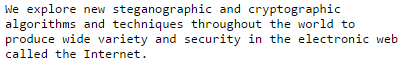
\includegraphics[scale=1]{Gambar/S0}
	\caption{Kalimat awal (S0)} 
	\label{fig:1-S0}
\end{figure}

lalu setelah disembunyikan suatu pesan dengan menggunakan \textit{line-shift coding}, muncul kalimat S1.

\begin{figure}[H]
	\centering
	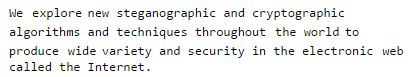
\includegraphics[scale=1]{Gambar/S1}
	\caption{Kalimat setelah melalui proses \textit{line-shift coding} (S1)} 
	\label{fig:2-S1}
\end{figure}

Dengan menumpukkan kedua kalimat S0 dan S1, didapatkan hasil sebagai berikut:

\begin{figure}[H]
	\centering
	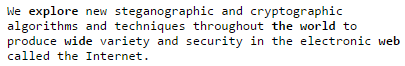
\includegraphics[scale=1]{Gambar/overlap-result}
	\caption{Hasil penumpukkan kalimat S0 dan S1} 
	\label{fig:2-overlap-result}
\end{figure}

Hasil ini dapat dicapai dengan melebarkan spasi sebelum kata \textit{explore}, \textit{the}, \textit{wide}, dan \textit{web}, juga menyempitkan spasi setelah kata \textit{explore}, \textit{world}, \textit{wide}, dan \textit{web} pada S1. Dengan demikian, kalimat yang mengandung \textit{shifted-word} akan tetap memiliki arti yang sama.

\subsubsection{Feature Coding}

\textit{Feature coding} memanfaatkan ciri yang ada dalam teks yang dapat diubah. Seperti garis lurus yang ada pada huruf b, d, h, k ,dan lain-lain. Panjang dari garis tersebut dapat diubah tanpa membuat curiga pembaca pada umumnya. Dapat juga dilakukan subtitusi pada beberapa kata dengan kata sinonimnya. Dengan itu kita dapat menyisipkan informasi 0 pada sinonim pertama dan 1 pada sinonim kedua. Cara ini harus melalui kesepakatan antara dua belah pihak tentang pasangan sinonimnya.

\subsubsection{Inter-sentence Spacing}

Cara ini akan menyandikan teks yang sudah dalam bentuk biner ke dalam teks dengan menyisipkan satu atau dua spasi setelah tiap kalimat. Misalkan satu spasi menyandikan 0 dan dua spasi menyandikan 1. Sayangnya cara ini memiliki beberapa masalah, yang pertama jika ingin menyisipkan teks yang memiliki ukuran yang besar, akan membutuhkan teks cover yang banyak pula karena 1 kalimat hanya dapat menyandikan 1 bit. Kedua, beberapa perangkat pengolah kata secara otomatis mengubah banyaknya spasi menjadi satu.

\subsubsection{End of Line Spacing}

Cara ini menyisipkan spasi pada akhir baris. Cara ini meningkatkan banyaknya informasi yang dapat disandikan dibandingkan cara sebelumnya. Sama seperti sebelumya, cara ini dapat terganggu oleh beberapa program yang dapat menghapus spasi yang berlebihan dari teks dan cara ini tidak dapat menampilkan pesan rahasia dari \textit{hard copy}.

\subsubsection{Inter-word Spacing}

Cara ketiga menggunakan spasi untuk menyandikan data yang menggunakan \textit{right-justification}. Data disandikan dengan mengatur di mana spasi ekstra akan diletakkan. Satu spasi di antara kata menyandikan 0 dan dua spasi menyandikan 1. Cara ini memungkinkan beberapa bit dapat disembunyikan dalam satu baris.

\subsection{Linguistic Steganography}
Metode ini memanfaatkan \textit{natural language processing} atau pemrosesan bahasa alami yang menyebabkan pesan dapat disembunyikan tanpa mengubah bahasa asli. Contohnya bisa dengan melakukan subtitusi terhadap sinonim yang termasuk steganografi leksikal. Perubahan dari kalimat aktif ke pasif atau sebaliknya untuk contoh dari sintaksis steganografi. Pemanfaatan suku kata untuk menyisipkan pesan yang juga termasuk ke dalam steganografi linguistik yang akan menjadi bahasan utama dalam skripsi ini.}{}
\ifdefstring{\vbabc}{1}{\chapter{Analisis}
Pada bab ini penulis akan membahas analisis masalah yang mungkin ada pada algoritma. Masalah yang mungkin akan dihadapi adalah beberapa kata yang ada pada \textit{stego cover} memiliki sinonim dengan banyak suku kata yang sama dengan kata aslinya(yang ada pada \textit{stego cover}). Selain itu juga \textit{stego cover} dapat berisi nama orang, sehingga tidak memiliki sinonim.

\section{Hipotesis}

\subsection{Pemenggalan Kata}
Untuk proses pemenggalan kata, akan menggunakan skripsi Frisca Sumarlin 2010 yang berjudul Aplikasi Pendongeng. Untuk mengenali suku kata dalam bahasa Indonesia, akan digunakan tiga tahap DFSA. Setiap masukan dari DFSA merupakan hasil DFSA tahap sebelumnya. Seperti yang telah dijelaskan , FSA memiliki prinsip kerja membaca hanya satu arah dan tidak bisa membaca mundur masukannya. Sedangkan untuk mengenali suku kata, untuk beberapa kasus kata dibutuhkan kemampuan untuk membaca mundur masukannya. Sebagai contoh, pada kata "anda", huruf ketiga adalah huruf konsonan sehingga pemenggalan suku kata dapat dilakukan pada saat membaca huruf ketiga. Berbeda dengan kata "anda", pada kata "alis", huruf ketiga adalah huruf vokal, \textit{automaton} harus mundur untuk melakukan pemenggalan suku kata.

Pada tahap 1 ini memang belum sesuai dengan aturan penyukuan kata yang benar, karena itu akan dilakukan tiga tahapan. Untuk diagramnya dapat dilihat pada gambar \ref{fig:1-DFSA-1}.

\begin{figure}[H]
	\centering
	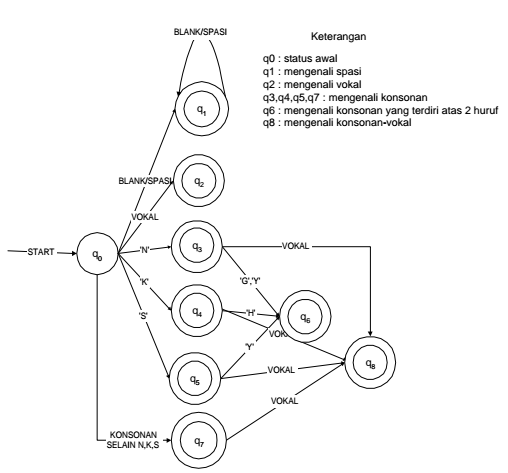
\includegraphics[scale=1.3]{Gambar/DFSA-1}
	\caption{Diagram Transisi DFSA tahap 1\cite{Thomas:2000}} 
	\label{fig:1-DFSA-1}
\end{figure}

Penjelasan tentang \ref{fig:1-DFSA-1}Diagram Transisi DFSA tahap 1 untuk mengenali spasi, vokal(V), konsonan yang terdiri dari 1 huruf (K), konsonan yang terdiri dari 2 huruf (KK), dan konsonan-vokal (KV) adalah sebagai berikut.

\begin{itemize}
	\item Perpindahan dari status awal (\textit{q0}) ke \textit{q1} adalah untuk mengenali spasi atau \textit{string} kosong.
	\item Perpindahan dari \textit{q0} ke \textit{q2} adalah untuk mengenali huruf vokal.
	\item Perpindahan dari \textit{q0} ke \textit{q3} adalah untuk mengenali huruf 'N'.
	\item Perpindahan dari \textit{q0} ke \textit{q4} adalah untuk mengenali huruf 'K'.
	\item Perpindahan dari \textit{q0} ke \textit{q5} adalah untuk mengenali huruf 'S'.
	\item Perpindahan dari \textit{q0} ke \textit{q7} adalah untuk mengenali huruf konsonan selain 'N', 'K', dan 'S'.
	\item Perpindahan dari \textit{q3} ke \textit{q8} adalah untuk mengenali pola suku kata VK.
	\item Perpindahan dari \textit{q3} ke \textit{q6} adalah untuk mengenali pola suku kata KK (ng dan ny).
	\item Perpindahan dari \textit{q3} ke \textit{q8} adalah untuk mengenali pola suku kata KV.
	\item Perpindahan dari \textit{q4} ke \textit{q6} adalah untuk mengenali pola suku kata KK (kh).
	\item Perpindahan dari \textit{q4} ke \textit{q8} adalah untuk mengenali pola suku kata KV.
	\item Perpindahan dari \textit{q5} ke \textit{q6} adalah untuk mengenali pola suku kata KK (sy).
	\item Perpindahan dari \textit{q5} ke \textit{q8} adalah untuk mengenali pola suku kata KV.
	\item Perpindahan dari \textit{q7} ke \textit{q8} adalah untuk mengenali pola suku kata KV.
\end{itemize}

Sebagai contoh, jika melakukan pemenggalan kata hanya dengan menggunakan \ref{fig:1-DFSA-1}DFSA tahap 1 saja, kata "gondok" tidak dapat dipotong secara sempurna. Berikut langkah-langkahnya.

\begin{itemize}
	\item Pada status awal (\textit{q0}) huruf ke-1 'g' akan diperiksa.
	\item Pindah ke \textit{q7} karena huruf 'g' merupakan huruf konsonan selain huruf 'N', 'K', dan 'S'.
	\item Huruf ke-2 'o' diperiksa dan pindah ke \textit{q8} karena huruf 'o' merupakan huruf vokal. Suku kata ke-1 "go" disimpan, lanjut ke huruf selanjutnya dan mulai lagi dari \textit{q0}.
	\item Huruf ke-3 'n' diperiksa dan pindah ke \textit{q3} karena huruf ke-3 adalah huruf 'n'.
	\item Huruf ke-4 'd' diperiksa dan tidak memenuhi syarat untuk ke \textit{q8} ataupun \textit{q6}. Suku kata ke-2 "n" disimpan. Huruf ke-4 'd' kembali ke \textit{q0}.
	\item Pindah ke \textit{q7} karena huruf 'd' merupakan huruf konsonan selain huruf 'N', 'K', dan 'S'.
	\item Huruf ke-5 'o' diperiksa dan pindah ke \textit{q8} karena '0' merupakan huruf vokal. Suku kata ke-3 "do" disimpan, lanjut ke huruf selanjutnya dan mulai lagi dari \textit{q0}.
	\item Huruf ke-6 'k' diperiksa dan pindah ke \textit{q4} karena huruf ke-6 adalah huruf 'K'. Suku kata ke-4 "k" disimpan. Tahap 1 selesai karena semua huruf telah melewati diagram transisi DFSA tahap 1.
	\item Didapatkan hasil pemenggalan suku kata "gondok" menjadi "go-n-do-k".
\end{itemize}

Dapat dilihat bahwa jika hanya menggunakan \ref{fig:1-DFSA-1}DFSA tahap 1, hasilnya masih belum sempurna. Pada tahan 1 hanya dikenali pola suku kata V, K, KV, dan KK. Selanjutnya, setelah melewati tahapan 1 DFSA, \textit{output}nya akan menjadi masukan untuk DFSA tahap 2. Pada tahap 2 ini harus dikenali V, KV, dan pengembangan dari ketiga pola yang dikenali pada tahap pertama. Pada tahap ini, pengembangan yang bisa dilakukan adalah V+K, K+KV, K+KV+K, K+K+KV, K+K+KV+K, K+KV+K, dan KV+K. Untuk digram transisi tahap kedua dapat dilihat pada gambar \ref{fig:2-DFSA-2}.

\begin{figure}[H]
	\centering
	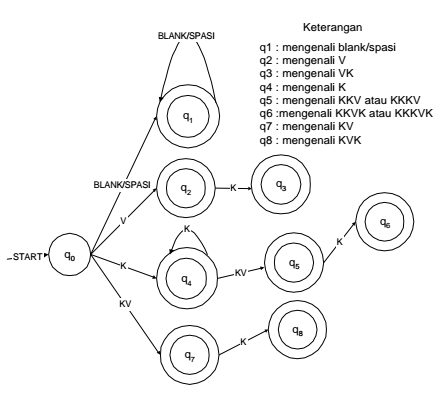
\includegraphics[scale=1.3]{Gambar/DFSA-2}
	\caption{Diagram Transisi DFSA tahap 2\cite{Thomas:2000} 
	\label{fig:2-DFSA-2}}
\end{figure}

Penjelasan tentang \ref{fig:1-DFSA-2}Diagram Transisi DFSA tahap 2 untuk mengenali pola suku kata V, VK, K, KKV, KKKV, KKVK, KKKVK, KV, dan KVK adalah sebagai berikut.

\begin{itemize}
	\item Perpindahan dari status awal (\textit{q0}) ke \textit{q1} adalah untuk mengenali spasi atau \textit{string} kosong.
	\item Perpindahan dari \textit{q0} ke \textit{q2} adalah untuk mengenali pola suku kata V.
	\item Perpindahan dari \textit{q0} ke \textit{q4} adalah untuk mengenali pola suku kata K.
	\item Perpindahan dari \textit{q0} ke \textit{q7} adalah untuk mengenali pola suku kata KV.
	\item Perpindahan dari \textit{q2} ke \textit{q3} adalah untuk mengenali pola suku kata VK.
	\item Perpindahan dari \textit{q4} ke \textit{q4} adalah untuk mengenali pola suku kata KK.
	\item Perpindahan dari \textit{q4} ke \textit{q5} adalah untuk mengenali pola suku kata KKV atau KKKV.
	\item Perpindahan dari \textit{q5} ke \textit{q6} adalah untuk mengenali pola suku kata KKVK atau KKKVK.
	\item Perpindahan dari \textit{q7} ke \textit{q8} adalah untuk mengenali pola suku kata KVK.
\end{itemize}

Pada tahap 2, masih ada tiga pola suku kata yang belum dapat dikenali, yaitu VKK, KVKK, dan KKVKK. Untuk itu masih dibutuhkan satu tahapan lagi untuk dapat mengenali pola-pola tersebut dan mengenali huruf diftong. Pada tahap ini hasil dari DFSA tahap kedua akan menjadi masukan bagi DFSA tahap terakhir yaitu tahap 3.

\begin{figure}[H]
	\centering
	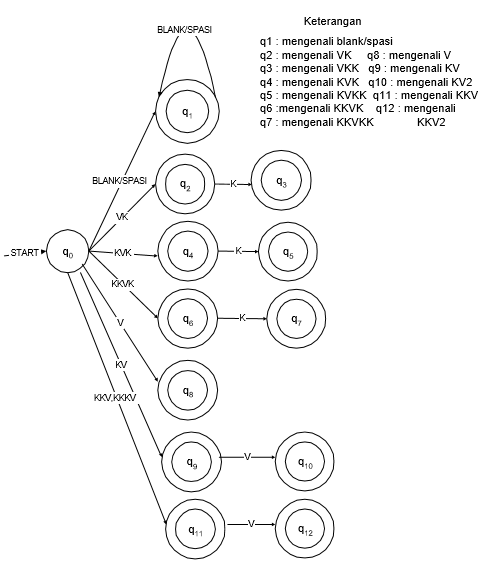
\includegraphics[scale=1.3]{Gambar/DFSA-3}
	\caption{Diagram Transisi DFSA tahap 3\cite{Thomas:2000}} 
	\label{fig:3-DFSA-3}
\end{figure}

Penjelasan tentang \ref{fig:1-DFSA-3}Diagram Transisi DFSA tahap 3 untuk mengenali pola suku kata VK, V, VKK, KV, KVK, KVV, KVKK, KKV, KKVK, KKVKK, dan KKVV adalah sebagai berikut.

\begin{itemize}
	\item Perpindahan dari status awal (\textit{q0}) ke \textit{q1} adalah untuk mengenali spasi atau \textit{string} kosong.
	\item Perpindahan dari \textit{q0} ke \textit{q2} adalah untuk mengenali pola suku kata VK.
	\item Perpindahan dari \textit{q0} ke \textit{q4} adalah untuk mengenali pola suku kata KVK.
	\item Perpindahan dari \textit{q0} ke \textit{q6} adalah untuk mengenali pola suku kata KKVK.
	\item Perpindahan dari \textit{q0} ke \textit{q8} adalah untuk mengenali pola suku kata V.
	\item Perpindahan dari \textit{q0} ke \textit{q9} adalah untuk mengenali pola suku kata KV.
	\item Perpindahan dari \textit{q0} ke \textit{q11} adalah untuk mengenali pola suku kata KKV atau KKKV.
	\item Perpindahan dari \textit{q2} ke \textit{q3} adalah untuk mengenali pola suku kata VKK.
	\item Perpindahan dari \textit{q4} ke \textit{q5} adalah untuk mengenali pola suku kata KVKK.
	\item Perpindahan dari \textit{q6} ke \textit{q7} adalah untuk mengenali pola suku kata KKVKK.
	\item Perpindahan dari \textit{q9} ke \textit{q10} adalah untuk mengenali pola suku kata KVV.
	\item Perpindahan dari \textit{q11} ke \textit{q12} adalah untuk mengenali pola suku kata KKVV atau KKKVV.
\end{itemize}

Untuk dapat membagi suku kata, diperlukan automata yang dapat menerima masukan berupa kata dan keluaran berupa suku kata. \textit{Finite State Transducer} merupakan \textit{finite state machine} yang memiliki dua pita, yaitu pita masukan dan pita keluaran. Automata yang telah dirancang adalah DFSA, di mana keluaran yang dihasilkan adalah dikenali atau tidak dikenali. Dengan merubah keluaran dari DFSA tersebut menjadi suku kata untuk setiap sekuens karakter yang telah dikenali, maka DFSA yang telah dirancang dapat dimanfaatkan untuk membagi kata menjadi suku kata. Atas dasar itu, DFSA dipilih untuk melakukan penyukuan kata.

Pemenggalan suku kata akan dipakai untuk mendapatkan banyak suku kata kata-kata yang terdapat pada \textit{stego cover}, sehingga dapat dihitung banyak suku kata tiap katanya. Namun karena kumpulan \textit{stego cover} yang akan dipakai dapat berupa cerita pendek(cerpen) atau puisi, maka isi dari \textit{stego cover} tidak hanya berupa kata-kata alfabet saja, tetapi juga ada angka yang bisa berupa tanggal, kata serapan, dan lain-lain. Hal ini kemudian dapat menjadi hambatan, karena seperti yang kita ketahui bahwa angka tidak memiliki suku kata. Hambatan lainnya juga datang dari kata-kata dalam bahasa asing dan singkatan.

Setelah menemui hambatan-hambatan di atas, akhirnya diputuskan beberapa solusi. Pertama-tama, dari keseluruhan isi \textit{stego cover}, tanda baca akan diabaikan(kecuali tanda penghubung '-'), sehingga yang akan dipenggal hanyalah kata-katanya saja. Semua angka akan dianggap sebagai satu suku kata. Semua singkatan atau kata dalam bahasa asing, akan dilakukan pemenggalan kata apa adanya.

\subsection{\textit{Database} kata}
Penyisipan akan memanfaatkan pasangan kata yang memiliki suku kata berbeda, namun memiliki arti yang sama atau serupa. \textit{Database} kata akan disimpan dalam sebuah \textit{file} dengan ekstensi .txt. Pada \textit{file} tersebut satu per satu kata yang ada pada \textit{stego cover} memiliki sinonimnya sendiri. Pencarian sinonim pertama-tama akan dicari pada Tesaurus. Tesaurus \footnote{http://kbbi.web.id/tesaurus}merupakan buku referensi berupa daftar kata dengan sinonimnya. Kata-kata yang terdaftar di Tesaurus adalah kata baku, sehingga jika pada \textit{stego cover} terdapat kata yang tidak dapat ditemukan pada Tesaurus, diperlukan penanganan tersendiri.

Solusinya adalah dengan mengubah-ubah imbuhan pada awal atau akhir kalimat, namun tetap memperhatikan konteks kalimat tersebut. Sebagai contoh, pada \textit{stego cover} terdapat kata 'menggendongnya', namun kata tersebut tidak dapat ditemukan pada Tesaurus, karena terdapat imbuhan. Sehingga untuk sinonimnya dapat digunakan kata 'menggendong'. Kedua kata tersebut memiliki jumlah suku kata yang berbeda, namun memiliki arti yang sama.

Terdapat beberapa kata yang memang tidak memiliki sinonim dengan jumlah suku kata yang berbeda. Kata 'lama' memiliki 2 suku kata, sedangkan sinonim yang ada pada Tesaurus adalah 'lamban' dan 'lelet'. Kedua sinonimnya memiliki suku kata yang genap, tetapi yang dibutuhkan adalah yang bersuku kata ganjil. Hal ini dapat diatasi dengan menyamarkannya sebagai \textit{typo} atau kesalahan pengetikkan. Contohnya dengan memasukkan kata 'lambaan' atau 'lamaa' sebagai sinonim dari kata 'lama'. Kata 'lambaan' dan 'lamaa', jika dipotong suku katanya dengan menggunakan pemotong suku kata yang telah dibuat, kedua kata tersebut memiliki suku kata ganjil.

\subsection{Stego Cover}
\textit{Stego cover} yang telah dikumpulkan berupa puisi dan cerpen. Alasan dipilihnya cerpen dan puisi sebagai \textit{stego cover}, karena puisi umumnya menggunakan satu kata berulang-ulang, sehingga dapat mengurangi banyaknya kata yang disimpan pada \textit{file database}. Sedangkan cerpen yang dipilih memiliki jumlah kata yang cukup banyak, ini menandakan kapasitas penyimpanan yang cukup besar.

Dengan dipilihnya cerpen dan puisi sebagai \textit{stego cover}, maka dibutuhkan skema komunikasi yang dapat menyamarkan artikel tersebut agar tidak menimbulkan kecurigaan oleh pihak lain. Skema komunikasi yang dipilih berupa komunikasi antara dua mahasiswa yang gemar mengirim puisi atau cerpen melalui \textit{email}. \textit{Email} yang dikirim mengandung \textit{stego object} yang merupakan hasil dari penyisipan \textit{secret message} pada \textit{stego cover}. Dengan skema komunikasi seperti ini, jika ada pihak lain yang membaca \textit{email} kedua mahasiswa tersebut, tidak akan mencurigai adanya kejanggalan karena kedua mahasiswa gemar berkirim puisi dan cerpen.

\subsection{Penyisipan}
Proses steganografi akan memanfaatkan suku kata dan sinonim kata itu sendiri. Ide utamanya adalah dengan mengganti kata-kata tertentu yang ada dalam \textit{stego cover} dengan kata-kata yang telah disediakan pada \textit{file database}. File \textit{database} berisi semua kata yang ada pada \textit{stego cover} berpasangan dengan sinonimnya. Pasangan kata yang ada pada \textit{database} merupakan sinonim dengan banyak suku kata yang berbeda(ganjil dan genap) dengan kata aslinya.

Penggantian kata pada \textit{stego cover} ditentukan dari ASCII \textit{secret message} yang akan disisipkan. ASCII\footnote{http://whatis.techtarget.com/definition/ASCII-American-Standard-Code-for-Information-Interchange} (\textit{American Standard Code for Information Interchange}) merupakan format yang paling umum untuk file teks yang ada di komputer dan internet. Kode ASCII yang akan dipakai direpresentasikan dengan 7-bit angka biner, yang berarti ada 7 digit angka 0 atau 1. Pemilihan 7-bit ini dikarenakan kode ASCII pada bilangan desimal hanya ada dari 0 sampai 127, sehingga jika menggunakan 8-bit, angka pertama(paling kiri) akan selalu bernilai 0. Dapat disimpulkan bahwa untuk menyisipkan 7-bit dibutuhkan 7 kata, 8-bit dibutuhkan 8 kata.  Untuk alasan memaksimalkan kapasitas penyisipan, maka diputuskan untuk merepresentasikan 1 karakter menjadi 7-bit.

Setelah \textit{secret message} diubah menjadi deretan kode ASCII, satu per satu digit kodenya akan dicocokkan dengan banyaknya suku kata pada \textit{stego cover}. Kode digit pertama akan disisipkan pada kata pertama \textit{stego cover}, digit kedua disisipkan pada kata kedua, dst. Jika banyak suku kata pada \textit{stego cover} tidak sesuai dengan kode, maka kata tersebut akan dicari sinonimnya pada \textit{file database}, jika ditemukan kata dengan banyak suku kata yang sesuai dengan kode, maka kata tersebut akan diganti. Pemberitahuan akan muncul jika kata yang tidak sesuai kode tidak memiliki sinonim pada \textit{file database}.

\subsubsection{Algoritma}
Seperti yang telah dijelaskan sebelumnya, algoritma ini akan memanfaatkan kata yang ada pada \textit{stego cover} untuk menyisipkan kode ASCII dari pesan rahasia. Proses penyisipan ini juga memanfaatkan \textit{file database} untuk mengubah kata asli yang ada pada \textit{stego cover} dengan kata sinonim yang ada pada \textit{file database} jika banyak suku kata tidak sesuai dengan kode ASCII pesan rahasia.

Algoritma penyisipan pesan rahasia pada \textit{stego cover} dengan memanfaatkan sinonim

\begin{enumerate}
	\item Meminta input berupa pesan rahasia(\textit{secret}).
	\item Tiap karakter pada \textit{secret} diubah menjadi kode ASCII 7-bit dan disimpan menjadi \textit{secret code}.
	\item Hitung berapa banyak angka yang ada pada \textit{secret code}.
	\item Cari \textit{stego cover} yang dapat menampung \textit{secret code}.(Banyaknya kata yang ada dalam \textit{stego cover} > banyak angka yang ada pada \textit{secret code}).
	\item Bangkitkan angka acak dari 0 sampai banyaknya \textit{stego cover} yang dapat menampung \textit{secret code}. Angka acak ini dinamakan \textit{random}.
	\item Buka file ke-\textit{random} dan baca per kata dengan mengabaikan tanda baca dan spasi.
	\item Untuk tiap kata ke-n, lakukan pemenggalan kata dan hitung banyaknya suku kata pada kata ke-n tersebut dan lakukan operasi \textit{mod} 2. Hasil operasi ini dinamakan banyakSK.
	\item Cocokkan banyakSK dengan angka ke-n yang ada pada \textit{secret code} secara berurutan.(banyakSK kata ke-n dicocokkan dengan angka ke-n \textit{secret code})
	\item Jika pada tahap 7 didapatkan banyakSK yang tidak sesuai dengan angka ke-n \textit{secret code}, lanjut ke tahap 9. Jika sesuai, ulangi tahap 7 sampai semua angka pada \textit{secret code} berhasil disisipkan.
	\item Cari sinonim kata tersebut pada \textit{file database}. Kata yang diambil hanya kata dengan banyakSK yang memiliki nilai berbeda.
	\item Dari kata-kata yang didapatkan dari tahap 10, akan dilakukan pengambilan kata secara acak.
	\item Kata yang telah diambil dari tahap 11, akan menggantikan kata yang tidak sesuai sebelumnya.
\end{enumerate}

\subsection{Ekstraksi Pesan Rahasia}
Pada proses pengekstraksian kembali pesan rahasia akan dibutuhkan input berupa \textit{stego-object} yang merupakan hasil dari penyisipan. Perangkat pertama-tama akan membaca secara keseluruhan inputnya, lalu melakukan pemenggalan kata sama seperti yang dilakukan pada saat proses penyisipan. Selesai melakukan pemenggalan kata, banyak suku kata tiap katanya akan dihitung dan dilakukan operasi \textit{mod} 2 sehingga didapatkan angka 0 dan 1. Saat ini telah didapatkan deretan angka 0 dan 1 yang dinamakan \textit{secret code}. Saat menyisipkan memang 1 karakter diubah menjadi kode ASCII 7-bit, namun \textit{java} menyediakan fungsi untuk mengubah deret biner 8-bit menjadi karakter. Sehingga untuk setiap 7-bit pada \textit{secret code} dapat ditambahkan angka 0 di paling kiri sebelum dijadikan \textit{input} pada fungsi \textit{java} tersebut.

Setelah selesai mengubah bit-bit yang ada menjadi karakter, hasilnya akan ditampilkan pada layar. Proses ektraksi ini melibatkan semua kata yang ada pada \textit{stego-object}, sehingga kata yang tidak disisipkan pesan rahasia pun ikut terekstraksi. Hasilnya pesan rahasia yang diekstrak, dapat menampilkan karakter-karakter yang tidak memiliki arti. Hal ini dibiarkan agar penerima \textit{stego-object} dapat mengekstraksi pesan rahasia tanpa memerlukan informasi apapun. Alasan lainnya juga agar \textit{stego cover} dapat memaksimalkan kapasitas penyisipan.

\section{Analisis Use Case}

Diagram \textit{use case} perangkat lunak steganografi ini memiliki satu aktor, yaitu pengguna. Berikut diagram \textit{usecase} dari perangkat lunak yang akan dibangun.

\begin{figure}[H]
	\centering
	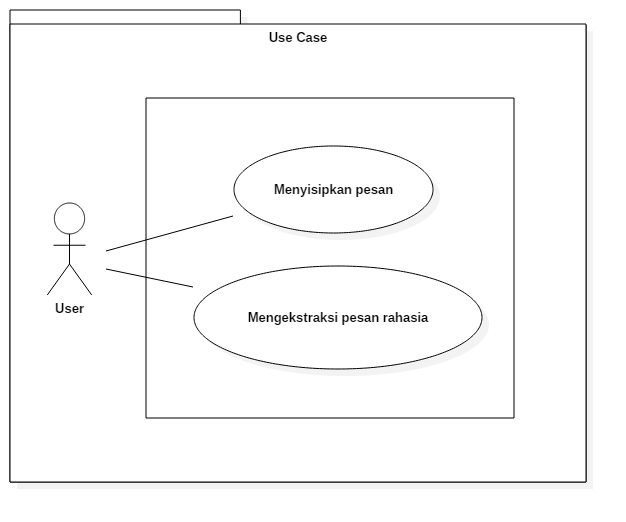
\includegraphics[scale=0.5]{Gambar/usecase}
	\caption{Use Case Diagram Perangkat Lunak Steganografi} 
	\label{fig:3_usecase}
\end{figure}

Dari diagram di atas dapat dilihat dua \textit{use case}, yakni:
\begin{enumerate}
	\item \textbf{Menyisipkan pesan}, pengguna mengetikkan pesan rahasia yang akan disisipkan.
	\item \textbf{Mengekstraksi kembali pesan rahasia}, pengguna akan memasukkan \textit{stego-object} yang diterima.
\end{enumerate}

\subsection{Skenario Use Case}

\begin{enumerate}
	\item \textbf{Menyisipkan pesan}
	\begin{itemize}
		\item Nama: Menyisipkan pesan
		\item Aktor: Pengguna
		\item Deskripsi: Mengetikkan pesan rahasia yang akan disisipkan		
		\item Prakondisi: -
		\item Tujuan: Menyisipkan pesan rahasia yang diketikkan ke dalam salah satu dokumen yang ada di dalam dokumen korpus
		\item Skenario:
			\begin{enumerate}
				\item Pengguna mengetikkan pesan rahasia yang akan disisipkan
				\item Pengguna menekan tombol sisipkan
				\item Sistem lalu akan mengubah pesan yang diketik menjadi kode ASCII
				\item Sistem mencari dokumen yang cocok dengan kode ASCII pesan rahasia
				\item \textit{Stego-object} sebagai hasil dari penyisipan akan muncul pada layar.
			\end{enumerate}
	\end{itemize}
	
	\item \textbf{Mengekstraksi pesan rahasia}
	\begin{itemize}
		\item Nama: Mengekstraksi pesan rahasia
		\item Aktor: Pengguna
		\item Deskripsi: Memasukkan \textit{stego-object} yang didapatkan
		\item Prakondisi: Telah memiliki \textit{stego-object} yang dihasilkan dari perangkat lunak ini
		\item Tujuan: Mengkestraksi pesan rahasia yang telah disisipkan sebelumnya
		\item Skenario:
			\begin{enumerate}
				\item Pengguna menyalin \textit{stego-object} yang didapat dari perangkat yang sama
				\item Pengguna menekan tombol Ekstrak
				\item Sistem akan melakukan penyukuan kata
				\item Masing-masing kata akan dijumlahkan suku katanya
				\item Sistem menyandikan jumlah suku kata yang genap menjadi 0 dan yang ganjil menjadi 1
				\item Sistem akan mengubah deret biner menjadi karakter yang sesuai dengan kode ASCII
				\item Pesan rahasia akan ditampilkan pada layar
			\end{enumerate}
	\end{itemize}
\end{enumerate}

\subsection{Analisis Diagram Kelas}

Diagram kelas perangkat lunak steganografi dapat dilihat pada \ref{fig:3_classdiagram}

\begin{figure}[H]
	\centering
	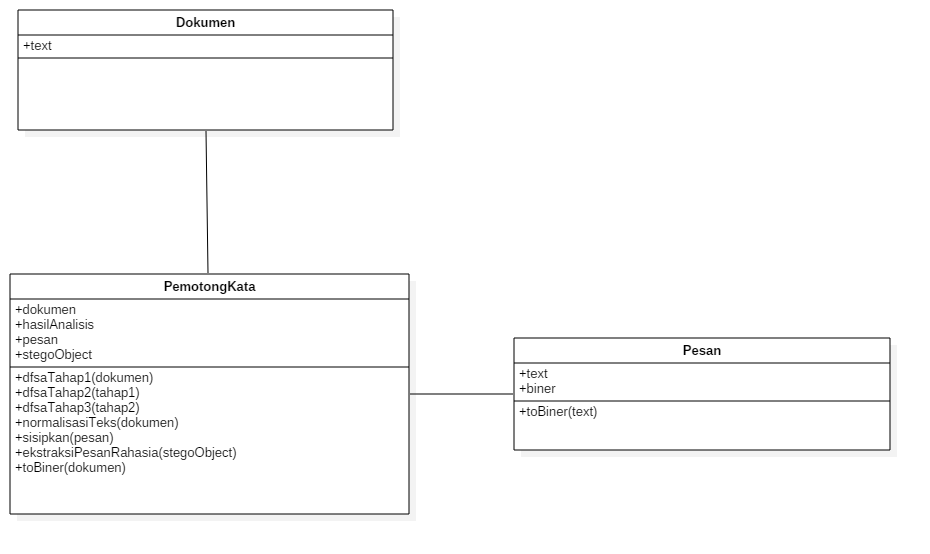
\includegraphics[scale=0.5]{Gambar/classdiagram}
	\caption{Class Diagram perangkat lunak steganografi} 
	\label{fig:3_classdiagram}
\end{figure}

Keterangan atas diagram kelas akan dijelaskan sebagai berikut:

\begin{enumerate}
	\item \textbf{Kelas Dokumen}
	\begin{itemize}
		\item Atribut text, untuk menampung teks dari dokumen berupa string
	\end{itemize}
	\item \textbf{Kelas Pesan}
	\begin{itemize}
		\item Atribut text, untuk menampung teks dari pesan berupa string
		\item Atribut biner, untuk menampung teks dari pesan berupa biner, tetapi dalam bentuk string
		\item Fungsi toBiner, memiliki parameter text. Fungsi ini akan merubah tiap karakter yang ditampung di atribut text menjadi kode ASCII dalam bentuk biner.
	\end{itemize}
	\item \textbf{Kelas PemotongKata}
	\begin{itemize}
		\item Atribut dokumen, untuk menampung isi dokumen
		\item Atribut hasilAnalisis, untuk menyimpan hasil dari penyukuan kata
		\item Atribut pesan, untuk menyimpan pesan rahasia yang akan disisipkan
		\item Atribut stegoObject, untuk menyimpan stego-object yang akan diektraksi
		\item Fungsi dfsaTahap1, memiliki parameter dokumen menghasilkan keluaran berupa hasil proses dfsa tahap pertama
		\item Fungsi dfsaTahap2, memiliki parameter tahap1 yang merupakan keluaran dfsaTahap1 dan mengeluarkan hasil proses dfsa tahap kedua
		\item Fungsi dfsaTahap3, memiliki parameter tahap2 yang merupakan keluaran dfsaTahap2 dan mengeluarkan hasil penyukuan kata dari text
		\item Fungsi normalisasiText, memiliki parameter dokumen dan menghasilkan keluaran berupa teks tanpa tanda baca dan simbol, sehingga siap untuk dipotong berdasarkan suku katanya
		\item Fungsi sisipkan, memiliki parameter pesan yang merupakan pesan rahasia yang diketikkan oleh pengguna dan akan mengeksekusi rangkaian penyisipan pesan
		\item Fungsi ekstraksiPesanRahasia, memiliki parameter stegoObject yang merupakan \textit{stego-object} yang disalin oleh pengguna dari hasil penyisipan menggunakan perangkat lunak yang sama dan akan mengeksekusi rangkaian pengekstraksian kembali pesan rahasia
		\item Fungsi toBiner, memiliki parameter dokumen. Parameter dokumen merupakan dokumen yang telah dilakukan penyukuan, sehingga fungsi ini hanya menghitung jumlah suku kata untuk setiap katanya. Jumlah kata akan disandikan dengan 0 untuk jumlah genap dan 1 untuk jumlah ganjil
	\end{itemize}
	
\end{enumerate}

\subsection{Analisis Diagram Aktivitas}

Diagram aktivitas dari perangkat lunak dibagi menjadi dua. Diagram aktivitas saat menyisipkan pesan dapat dilihat pada \ref{fig:4_activity-penyisipan}

\begin{figure}[H]
	\centering
	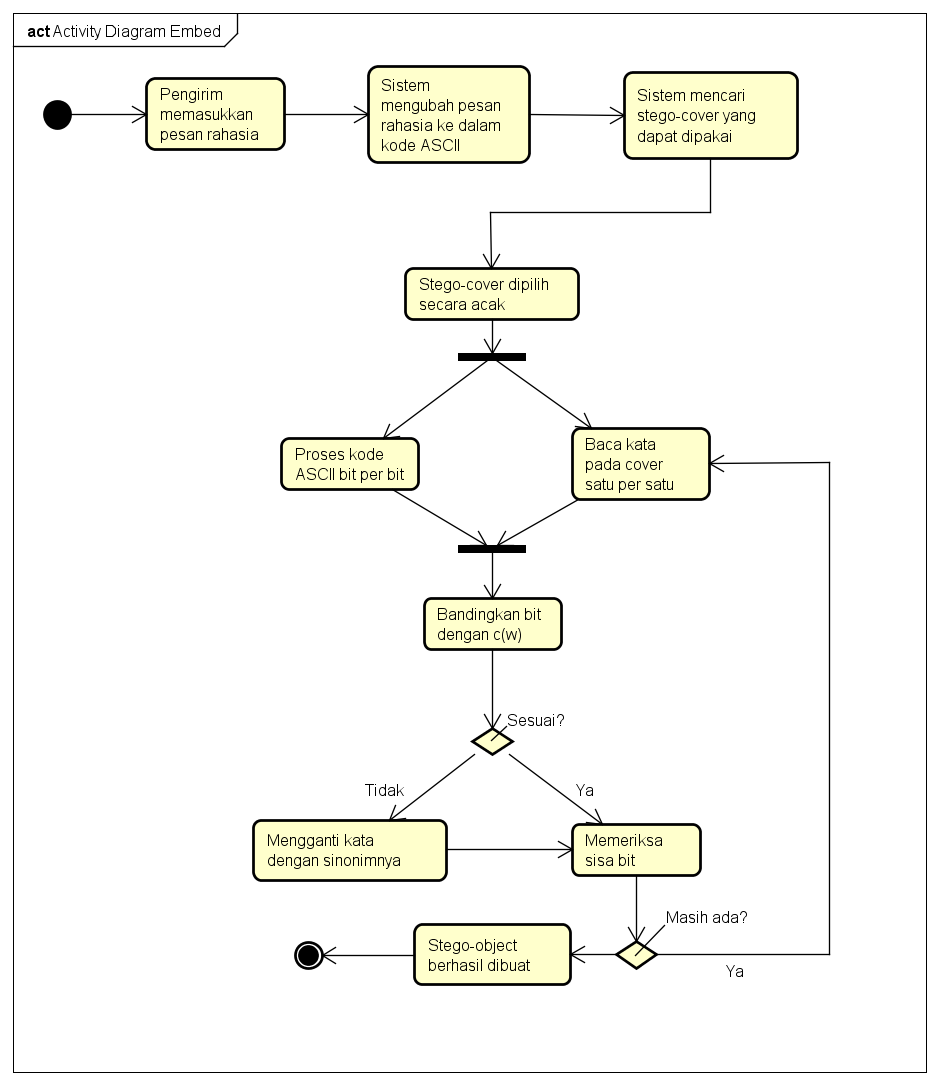
\includegraphics[scale=0.5]{Gambar/activity-penyisipan}
	\caption{Activity Diagram perangkat lunak steganografi saat menyisipkan} 
	\label{fig:4_activity-penyisipan}
\end{figure}

Dari diagram aktivitas dapat dijelaskan sebagai berikut:

\begin{enumerate}
	\item Pengguna memasukkan input berupa string (pesan rahasia)
	\item Pesan akan diubah ke bentuk ASCII
	\item Dokumen korpus akan dibuka satu per satu
	\item Untuk setiap dokumen yang dibuka akan dilakukan penyukuan kata dan dilakukan penyandian. Angka 1 untuk kata dengan jumlah suku kata genap dan angka 2 untuk kata dengan jumlah suku kata ganjil
	\item Pesan rahasia yang telah diubah ke bentuk ASCII dan dokumen yang telah disandikan akan dibandingkan. Dari sini akan dihasilkan dua kemungkinan:
	\begin{itemize}
		\item Jika ditemukan dokumen cocok dengan pesan rahasia, akan diambil kalimat yang sesuai
		\item Jika tidak ditemukan dokumen yang cocok, dari dokumen yang paling mirip akan dilakukan modifikasi (perubahan sinonim atau perubahan kalimat aktif/pasif)
	\end{itemize}
	\item Jika telah didapatkan kalimat yang sesuai, kalimat akan ditampilkan dan program selesai
\end{enumerate}

Diagram aktivitas ekstraksi dapat dilihat pada 

\begin{figure}[H]
	\centering
	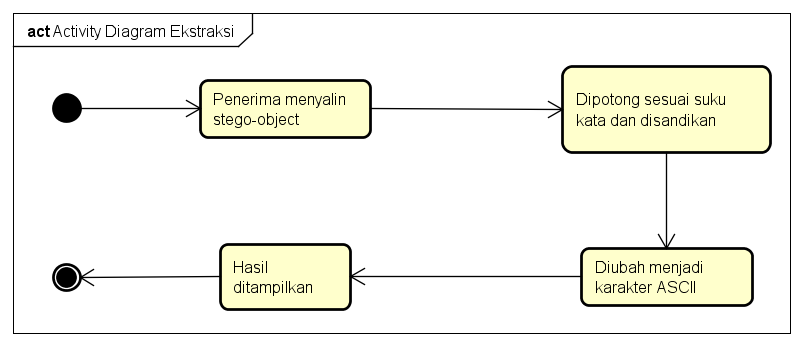
\includegraphics[scale=0.5]{Gambar/activity-ekstraksi}
	\caption{Activity Diagram perangkat lunak steganografi saat proses ekstraksi} 
	\label{fig:4_activity-ekstraksi}
\end{figure}

Dari diagram aktivitas di atas dapat dijelaskan sebagai berikut:

\begin{enumerate}
	\item Pengguna akan memberikan input berupa stego-object dari program yang sama
	\item Sistem lalu akan menyukukan kata-kata yang ada. Setelah itu dilakukan penyandian, angka 0 untuk kata dengan jumlah suku kata genap dan angka 1 untuk jumlah ganjil
	\item Selesai melakukan penyandian, hasilnya akan diubah menjadi karakter ASCII yang sesuai
	\item Kini sudah didapatkan pesan dengan karakter ASCII, hasil akan ditampilkan pada layar
\end{enumerate}}{}
\ifdefstring{\vbabd}{1}{\chapter{Perancangan}
Bab ini akan membahas mengenai perancangan aplikasi. Perancangan aplikasi akan meliputi tampilan antarmuka, diagram kelas lengkap beserta dengan deskripsi dan fungsinya.

\section{Perancangan Antarmuka}

Agar pengguna dapat menggunakan perangkat lunak ini dengan nyaman, maka dibutuhkan antarmuka. Rancangan antarmuka yang dibuat terdiri dari satu \textit{frame} dan di dalamnya terdapat beberapa \textit{tab}.

\subsection{\textit{Tab Embed}}

\begin{figure}[H]
	\centering
	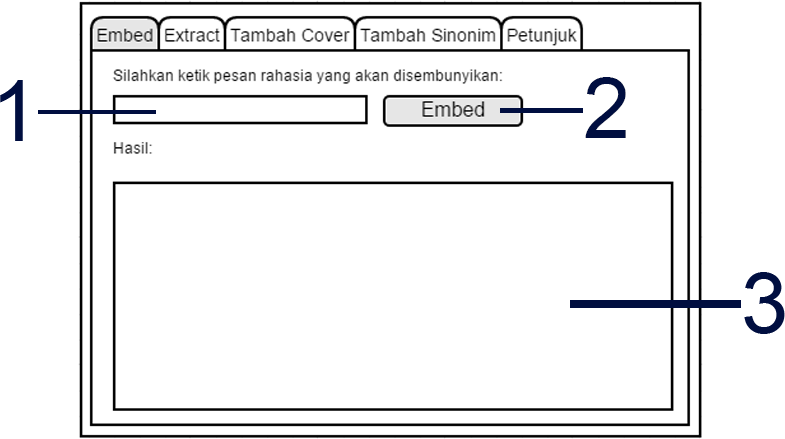
\includegraphics[scale=1.8]{Gambar/tab-embed}
	\caption{Tampilan \textit{tab Embed}} 
	\label{fig:1-tab-embed}
\end{figure}

Pada \textit{tab Embed} (dapat dilihat pada Gambar \ref{fig:1-tab-embed}) terdapat beberapa elemen sebagai berikut.

\begin{enumerate}
	\item \textbf{\textit{Text box secret message}}, pengguna dapat mengetikkan pesan rahasia yang akan disembunyikan pada bagian ini.
	\item \textbf{Tombol \textit{Embed}}, pengguna dapat menekan tombol ini untuk melakukan proses \textit{embedding}.
	\item \textbf{\textit{Text area stego-object}}, hasil proses \textit{embedding} yang merupakan \textit{stego-object} akan muncul pada bagian ini.
\end{enumerate}

\subsection{\textit{Tab Extract}}

\begin{figure}[H]
	\centering
	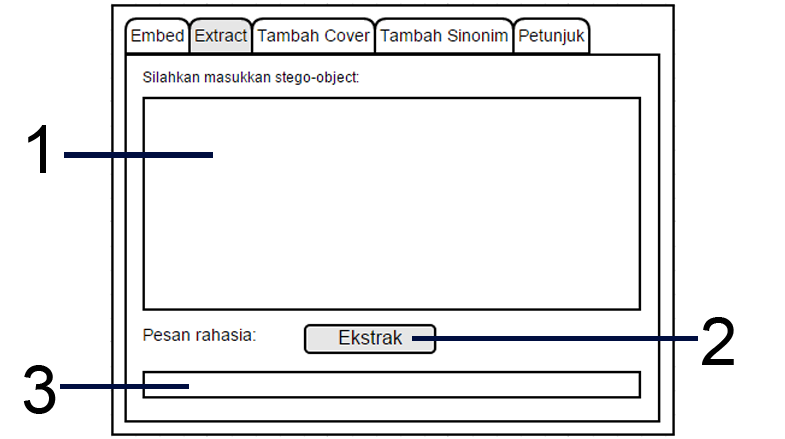
\includegraphics[scale=1.8]{Gambar/tab-extract}
	\caption{Tampilan \textit{tab Extract}} 
	\label{fig:2-tab-extract}
\end{figure}

Pada \textit{tab Extract} (dapat dilihat pada Gambar \ref{fig:2-tab-extract}) terdapat beberapa elemen sebagai berikut.

\begin{enumerate}
	\item \textbf{\textit{Text area stego-object}}, pengguna dapat menyalin \textit{stego-object} yang diterima pada bagian ini.
	\item \textbf{Tombol Ekstrak}, pengguna dapat menekan tombol ini untuk melakukan proses \textit{extracting}.
	\item \textbf{\textit{Text box secret message}}, hasil \textit{extracting} akan ditampilkan pada bagian ini.
\end{enumerate} 

\subsection{\textit{Tab} Tambah \textit{Cover}}

\begin{figure}[H]
	\centering
	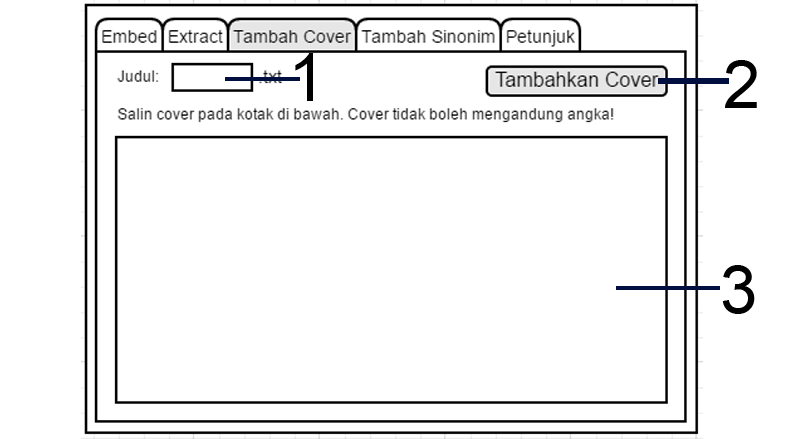
\includegraphics[scale=1.8]{Gambar/tab-tambah-cover}
	\caption{Tampilan \textit{tab} Tambah \textit{Cover}} 
	\label{fig:3-tab-tambah-cover}
\end{figure}

Pada \textit{tab} Tambah \textit{Cover} (dapat dilihat pada Gambar \ref{fig:3-tab-tambah-cover}) terdapat beberapa elemen sebagai berikut.

\begin{enumerate}
	\item \textbf{\textit{Text box} judul}, pengguna dapat mengetikkan judul dari \textit{stego-cover} yang akan ditambahkan pada bagian ini.
	\item \textbf{Tombol Tambah \textit{Cover}}, pengguna dapat menekan tombol ini untuk menambahkan \textit{stego-cover} yang telah disalin pada no 3.
	\item \textbf{\textit{Text area stego-cover}}, pengguna dapat menyalin \textit{stego-cover} yang memenuhi persyaratan di bagian ini.	
\end{enumerate} 

\subsection{\textit{Tab} Tambah Sinonim}

\begin{figure}[H]
	\centering
	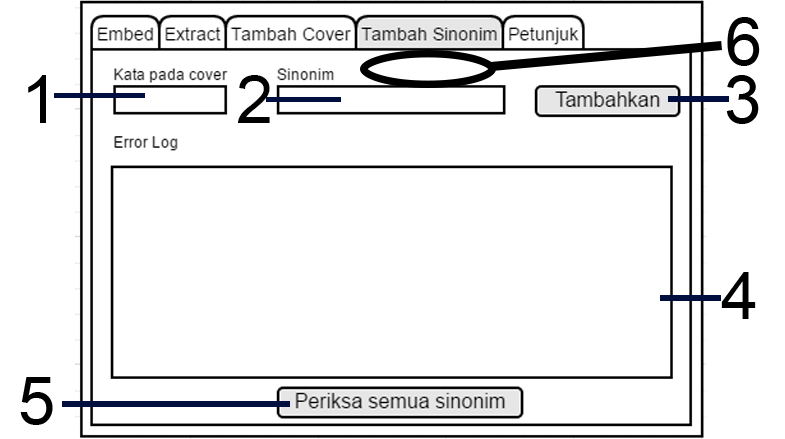
\includegraphics[scale=1.8]{Gambar/tab-tambah-sinonim}
	\caption{Tampilan \textit{tab} Tambah Sinonim} 
	\label{fig:4-tab-tambah-sinonim}
\end{figure}

Pada \textit{tab} Tambah Sinonim (dapat dilihat pada Gambar \ref{fig:4-tab-tambah-sinonim}) terdapat beberapa elemen sebagai berikut.

\begin{enumerate}
	\item \textbf{\textit{Text box} kata pada \textit{cover}}, kata pada \textit{cover} berarti kata yang ada pada \textit{stego-cover}, pengguna dapat mengetikkannya pada bagian ini.
	\item \textbf{\textit{Text box} sinonim}, pengguna dapat mengetik sinonimnya pada bagian ini.
	\item \textbf{Tombol Tambahkan}, pengguna dapat menekan tombol ini untuk memasukkan pasangan kata dan sinonim yang baru ke \textit{file database}.
	\item \textbf{\textit{Text Area} Error Log}, akan menampilkan daftar kata yang belum memiliki sinonim jika pengguna menekan tombol Periksa semua sinonim.
	\item \textbf{Tombol Periksa semua sinonim}, akan memeriksa semua kata dari tiap \textit{stego-cover} yang terdaftar dan menampilkan daftar kata yang belum memiliki sinonim.
\end{enumerate} 

\subsection{\textit{Tab} Petunjuk}

\begin{figure}[H]
	\centering
	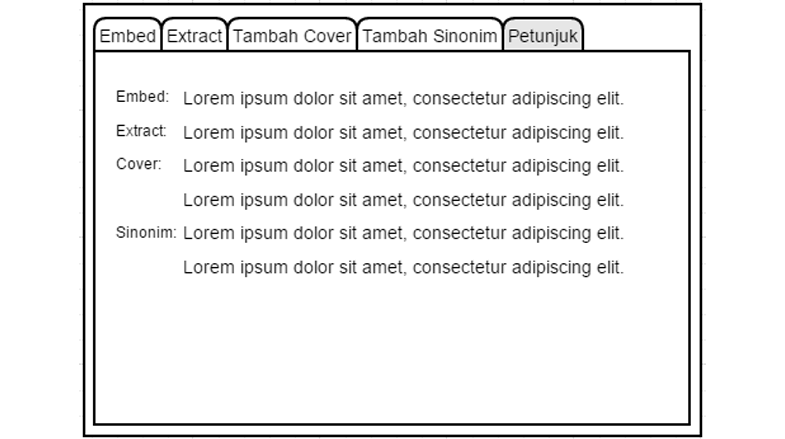
\includegraphics[scale=1.8]{Gambar/tab-petunjuk}
	\caption{Tampilan \textit{tab} Petunjuk} 
	\label{fig:5-tab-petunjuk}
\end{figure}

\textit{Tab} Petunjuk (dapat dilihat pada Gambar \ref{fig:5-tab-petunjuk}) sebenarnya hanya dibuat untuk membantu pengguna yang baru pertama kali memakai perangkat lunak ini. Pada \textit{tab} ini berisi petunjuk-petunjuk yang dapat membantu pengguna untuk mengoperasikan perangkat lunak ini.

\section{Diagram Kelas Rinci}

Diagram kelas sebelumnya yang dapat dilihat pada Gambar \ref{fig:3_classdiagram} mengalami beberapa perubahan dan penambahan kelas.

\section{Analisis Diagram Aktivitas}

Diagram aktivitas dari perangkat lunak dibagi menjadi dua. Diagram aktivitas saat menyisipkan pesan dapat dilihat pada \ref{fig:4_activity-penyisipan}

\begin{figure}[H]
	\centering
	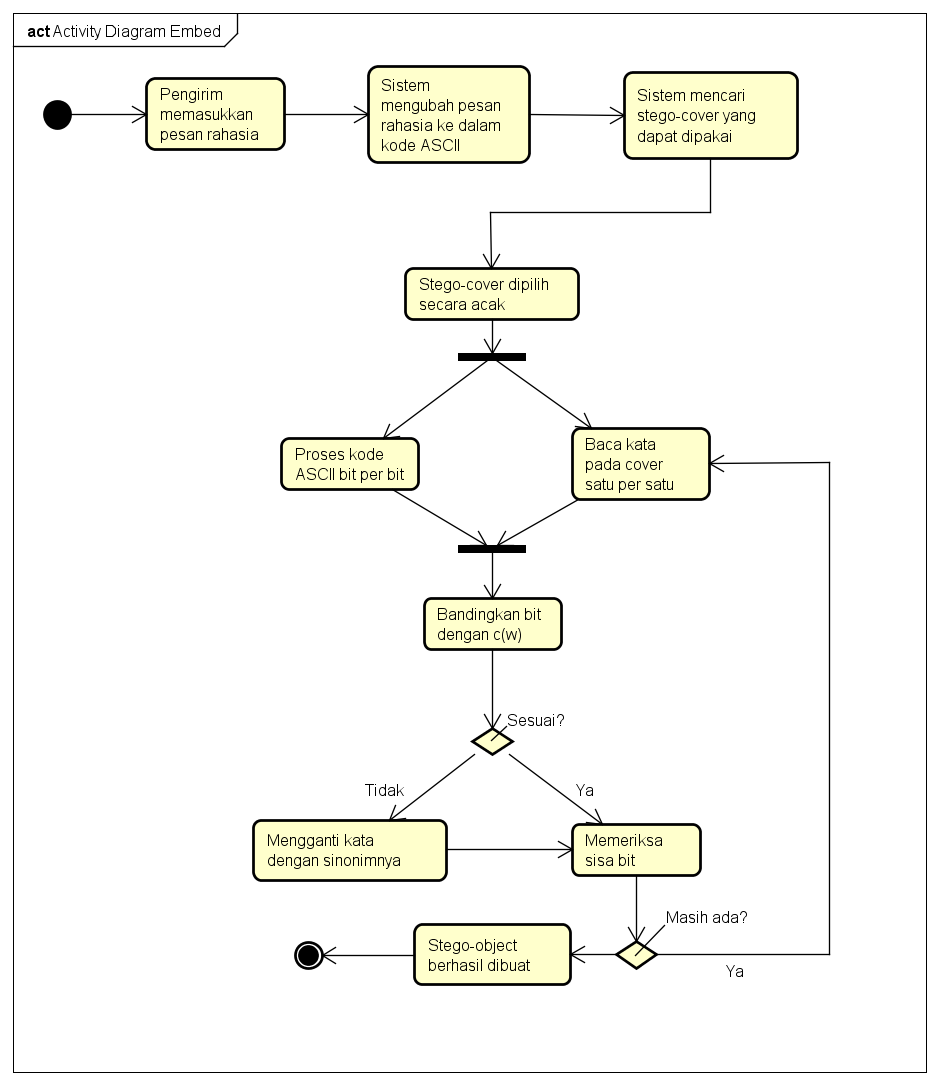
\includegraphics[scale=0.5]{Gambar/activity-penyisipan}
	\caption{Activity Diagram perangkat lunak steganografi saat menyisipkan} 
	\label{fig:4_activity-penyisipan}
\end{figure}

Dari diagram aktivitas dapat dijelaskan sebagai berikut:

\begin{enumerate}
	\item Pengguna memasukkan input berupa string (pesan rahasia)
	\item Pesan akan diubah ke bentuk ASCII
	\item Dokumen korpus akan dibuka satu per satu
	\item Untuk setiap dokumen yang dibuka akan dilakukan penyukuan kata dan dilakukan penyandian. Angka 1 untuk kata dengan jumlah suku kata genap dan angka 2 untuk kata dengan jumlah suku kata ganjil
	\item Pesan rahasia yang telah diubah ke bentuk ASCII dan dokumen yang telah disandikan akan dibandingkan. Dari sini akan dihasilkan dua kemungkinan:
	\begin{itemize}
		\item Jika ditemukan dokumen cocok dengan pesan rahasia, akan diambil kalimat yang sesuai
		\item Jika tidak ditemukan dokumen yang cocok, dari dokumen yang paling mirip akan dilakukan modifikasi (perubahan sinonim atau perubahan kalimat aktif/pasif)
	\end{itemize}
	\item Jika telah didapatkan kalimat yang sesuai, kalimat akan ditampilkan dan program selesai
\end{enumerate}

Diagram aktivitas ekstraksi dapat dilihat pada 

\begin{figure}[H]
	\centering
	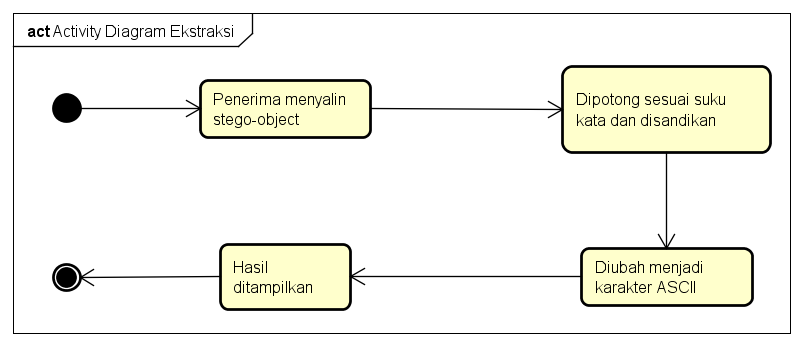
\includegraphics[scale=0.5]{Gambar/activity-ekstraksi}
	\caption{Activity Diagram perangkat lunak steganografi saat proses ekstraksi} 
	\label{fig:4_activity-ekstraksi}
\end{figure}

Dari diagram aktivitas di atas dapat dijelaskan sebagai berikut:

\begin{enumerate}
	\item Pengguna akan memberikan input berupa stego-object dari program yang sama
	\item Sistem lalu akan menyukukan kata-kata yang ada. Setelah itu dilakukan penyandian, angka 0 untuk kata dengan jumlah suku kata genap dan angka 1 untuk jumlah ganjil
	\item Selesai melakukan penyandian, hasilnya akan diubah menjadi karakter ASCII yang sesuai
	\item Kini sudah didapatkan pesan dengan karakter ASCII, hasil akan ditampilkan pada layar
\end{enumerate}}{}
\ifdefstring{\vbabe}{1}{\chapter{Implementasi dan Pengujian}
Bab ini akan berisi tentang implementasi perangkat lunak serta pengujian pada perangkat lunak tersebut. Hasil dari pengujian akan digunakan untuk menarik kesimpulan. 

\section{Implementasi}
Perangkat lunak akan diimplementasikan menjadi sebuah program dengan menggunakan bahasa Java. Rancangan antarmuka yang telah dijelaskan pada Bab \ref{perancangan_antarmuka}, telah berhasil diimplementasikan dan dapat dilihat pada gambar-gambar di bawah ini.

\begin{figure}[H]
	\centering
	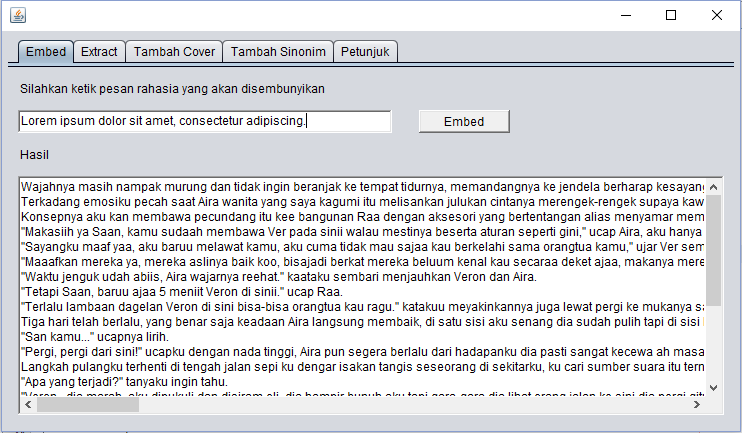
\includegraphics[scale=0.8]{Gambar/ui-embed}
	\caption{Tampilan \textit{tab Embed}} 
	\label{fig:ui-embed}
\end{figure}

\begin{figure}[H]
	\centering
	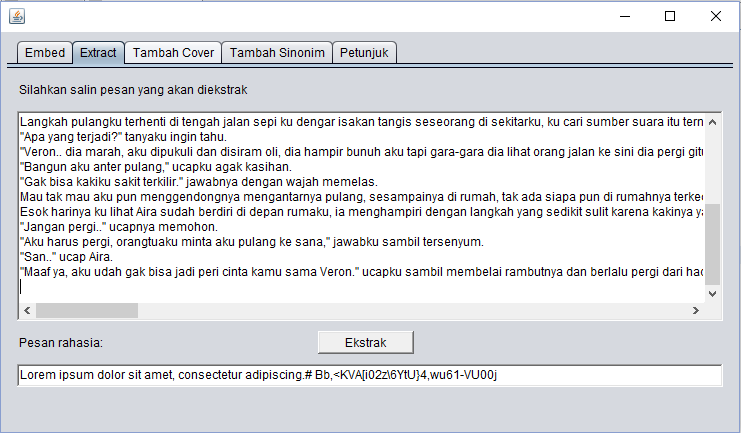
\includegraphics[scale=0.8]{Gambar/ui-extract}
	\caption{Tampilan \textit{tab Extract}} 
	\label{fig:ui-extract}
\end{figure}

Gambar \ref{fig:ui-extract} menunjukkan bahwa ada karakter '\#' yang memberitahu penerima bahwa pesan rahasia telah berakhir, seperti yang telah dijelaskan pada Bab \ref{algoritma}.

\begin{figure}[H]
	\centering
	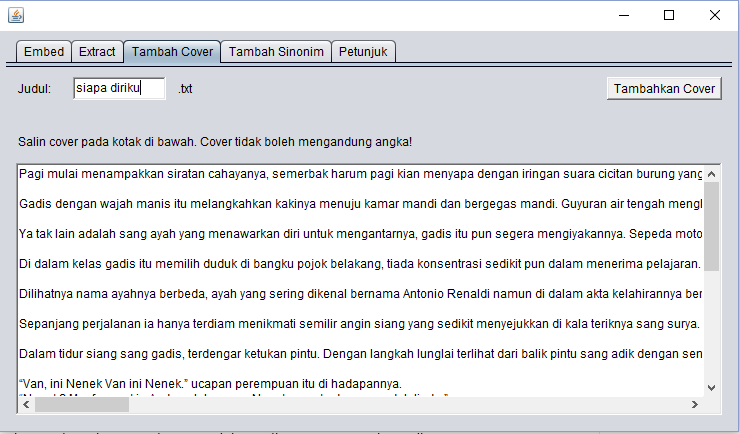
\includegraphics[scale=0.8]{Gambar/ui-tambah-cover}
	\caption{Tampilan \textit{tab Tambah Cover}} 
	\label{fig:ui-tambah-cover}
\end{figure}

\begin{figure}[H]
	\centering
	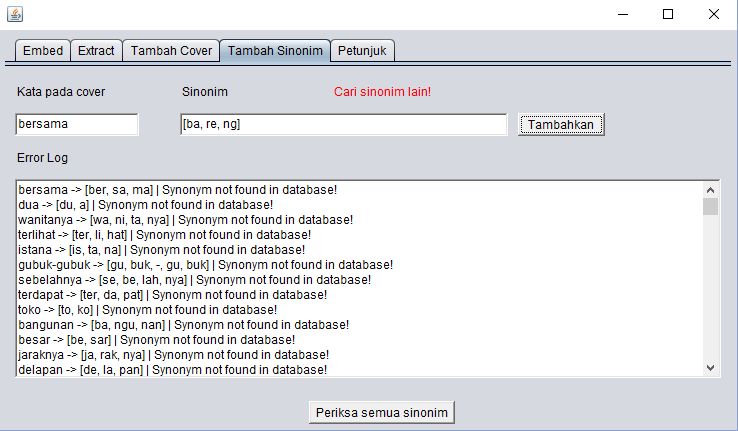
\includegraphics[scale=0.8]{Gambar/ui-tambah-sinonim}
	\caption{Tampilan \textit{tab Tambah Sinonim}} 
	\label{fig:ui-tambah-sinonim}
\end{figure}

Gambar \ref{fig:ui-tambah-sinonim} merupakan contoh saat pengirim memasukkan pasangan kata dan sinonim yang memiliki \textit{c}(\textit{w}) yang memiliki nilai yang sama. Seperti yang telah dijelaskan pada Bab \ref{perancangan_antarmuka}, jika penambahan sinonim gagal, \textit{textbox} sinonim akan diisi dengan hasil pemenggalan kata oleh perangkat lunak. Hal ini dilakukan untuk memberitahu pengirim bagaimana perangkat lunak memenggal kata tersebut. Pemenggalan kata yang dilakukan oleh perangkat lunak tidak sempurna, namun hal ini tidak menjadi masalah karena yang terpenting pemenggalan katanya konsisten.

\begin{figure}[H]
	\centering
	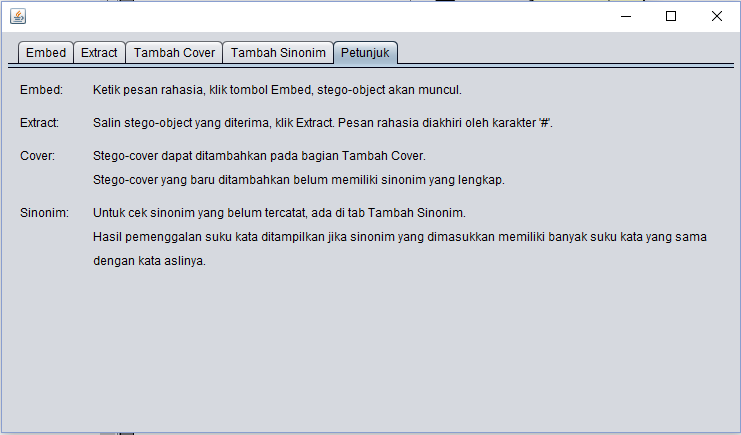
\includegraphics[scale=0.8]{Gambar/ui-petunjuk}
	\caption{Tampilan \textit{tab Petunjuk}} 
	\label{fig:ui-petunjuk}
\end{figure}

\section{Pengujian}
Pengujian yang dilakukan adalah pengujian fungsional dan pengujian eksperimental. Pengujian ini dilakukan untuk memeriksa apakah perangkat lunak yang dibuat telah berfungsi dengan baik. Hasil pengujian ini juga akan dipakai untuk menarik kesimpulan pada bab terakhir.

\subsection{Pengujian Fungsional}
Pengujian fungsional dilakukan untuk memeriksa apakah perangkat lunak memberikan reaksi yang seharusnya terhadap aksi dari pengguna perangkat lunak. Pengujian ini dilakukan pada sistem operasi Windows. Terdapat beberapa tes kasus yang diujikan kepada setiap fungsinya, untuk lengkapnya dapat dilihat pada tabel masing-masing di bawah ini.\\

\begin{table}[H]
\label{table-fungsional-embed}
\centering
\caption{Tabel Pengujian Fungsional \textit{Embed}}
\begin{tabular}{|p{0.3cm} | p{4.5cm} | p{7cm} | p{2.5cm} |}\hline
No. & Aksi & Reaksi seharusnya & Hasil\\
\hline
1 & Pengguna mengetikkan pesan rahasia sepanjang 100 karakter lalu menekan tombol Embed (panjang karakter pesan rahasia masih dapat ditampung \textit{stego-cover} yang ada.) & Perangkat lunak menampilkan \textit{stego-cover} & Sesuai\\
\hline
2 & Pengguna mengetikkan pesan rahasia sepanjang 200 karakter lalu menekan tombol Embed (panjang karakter pesan rahasia tidak dapat ditampung \textit{stego-cover} yang ada.) & Perangkat lunak menampilkan \textit{stego-cover} & Perangkat lunak menampilkan teks "Pesan rahasia melebihi kapasitas yang ada!"\\
\hline
3 & Pengguna mengetikkan pesan rahasia yang mengandung karakter yang tidak didukung perangkat lunak & Perangkat lunak menampilkan \textit{stego-cover} & Sesuai \\
\hline
\end{tabular}
\end{table}

\begin{table}[H]
\label{table-fungsional-extract}
\centering
\caption{Tabel Pengujian Fungsional \textit{Extract}}
\begin{tabular}{|p{0.3cm} | p{4.5cm} | p{7cm} | p{2.5cm} |}\hline
No. & Aksi & Reaksi seharusnya & Hasil\\
\hline
1 & Pengguna memasukkan \textit{stego-object} lalu menekan tombol Extract & Perangkat lunak menampilkan pesan rahasia, karakter '\#' menandakan pesan rahasia telah berakhir & Sesuai \\
\hline
2 & Pengguna memasukkan teks yang bukan \textit{stego-object} lalu menekan tombol Extract & Perangkat lunak menampilkan pesan bahwa tidak ada pesan rahasia dalam \textit{stego-object} yang dimasukkan & Sesuai \\
\hline
3 & Pengguna memasukkan \textit{stego-object} yang merupakan hasil \textit{embed} pesan rahasia yang mengandung karakter yang tidak didukung perangkat lunak & Perangkat lunak menampilkan pesan rahasia & Perangkat lunak menampilkan pesan rahasia namun tidak sesuai dengan pesan rahasia yang disembunyikan.\\
\hline
\end{tabular}
\end{table}

Pada Tabel \ref{table-fungsional-extract}, dapat dilihat bahwa pada nomor 3 menampilkan pesan rahasia yang tidak sesuai dengan yang disembunyikan. Hal tersebut terjadi karena saat proses \textit{embed}, karakter yang tidak terdaftar tersebut bisa saja memiliki ASCII yang lebih dari 7 bit, sehingga pada saat ekstraksi, hanya 7 bit pertama dari karakter tersebut yang diekstraksi. Hasilnya pesan yang diekstrak tidak sesuai. 

\begin{table}[H]
\label{table-fungsional-tambah-cover}
\centering
\caption{Tabel Pengujian Fungsional Tambah Cover}
\begin{tabular}{|p{0.3cm} | p{4.5cm} | p{7cm} | p{2.5cm} |}\hline
No. & Aksi & Reaksi seharusnya & Hasil\\
\hline
1 & Pengguna memasukkan \textit{stego-cover} dan judul yang belum terdaftar & Perangkat lunak membuat \textit{file stego-cover} yang baru dan mendaftarkannya pada \textit{stego-cover list} & Sesuai\\
\hline
2 & Pengguna memasukkan \textit{stego-cover} tanpa memasukkan judul & Perangkat lunak menampilkan pesan bahwa judul belum diisi & Sesuai \\
\hline
3 & Pengguna memasukkan \textit{stego-cover} dengan judul yang sudah terdaftar & Perangkat lunak menampilkan pesan bahwa judul sudah terdaftar & Sesuai \\
\hline
4 & Pengguna memasukkan judul yang belum terdaftar, tetapi \textit{stego-cover} yang dimasukkan sudah pernah ditambahkan & Perangkat lunak membuat \textit{file stego-cover} yang baru dan mendaftarkannya pada \textit{stego-cover list} & Sesuai \\
\hline
\end{tabular}
\end{table}

Pada Tabel \ref{table-fungsional-tambah-cover}, dapat dilihat bahwa untuk kasus pada nomor 4, \textit{stego-cover} tetap ditambahkan. Hal ini dikarenakan perangkat lunak hanya memeriksa apakah judul yang dimasukkan pengguna sudah terdaftar atau belum, tanpa memeriksa isi dari \textit{stego-cover} yang dimasukkan pengguna.

\begin{table}[H]
\label{table-fungsional-tambah-sinonim}
\centering
\caption{Tabel Pengujian Fungsional Tambah Sinonim}
\begin{tabular}{|p{0.3cm} | p{4.5cm} | p{7cm} | p{2.5cm} |}\hline
No. & Aksi & Reaksi seharusnya & Hasil \\
\hline
1 & Pengguna menambahkan kata dan sinonim dengan nilai \textit{c}(\textit{w}) yang berbeda & Perangkat lunak menambahkan sinonim ke kamus sinonim & Sesuai \\
\hline
2 & Pengguna menambahkan kata dan sinonim dengan nilai \textit{c}(\textit{w}) yang sama & Perangkat lunak menampilkan peringatan dan hasil pemenggalan sinonim & Sesuai \\
\hline
\end{tabular}
\end{table}

\begin{table}[H]
\label{table-fungsional-cek-sinonim}
\centering
\caption{Tabel Pengujian Fungsional Cek Semua Sinonim}
\begin{tabular}{|p{0.3cm} | p{4.5cm} | p{7cm} | p{2.5cm} |}\hline
No. & Aksi & Reaksi seharusnya & Hasil \\
\hline
1 & Pengguna memeriksa semua sinonim (ada kata yang sinonimnya belum terdaftar) & Perangkat lunak menampilkan kata-kata yang sinonimnya tidak terdaftar pada kamus sinonim & Sesuai\\
\hline
2 & Pengguna memeriksa semua sinonim (semua kata sudah terdaftar sinonimnya) & Perangkat lunak tidak menampilkan apa pun & Sesuai \\
\hline
\end{tabular}
\end{table}

\subsection{Pengujian Eksperimental}
Pengujian eksperimental ini dilakukan untuk meneliti waktu dari respon perangkat lunak terhadap beberapa kasus. Dapat dilihat pada Gambar \ref{fig:graf-embed} grafik perbandingan antara waktu yang dibutuhkan untuk \textit{embed} pesan rahasia yang pendek sampai yang panjang.

\begin{figure}[H]
	\centering
	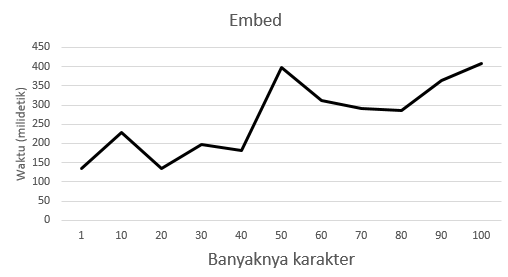
\includegraphics[scale=0.8]{Gambar/graf-embed}
	\caption{Grafik waktu yang dibutuhkan \textit{embed} pesan rahasia} 
	\label{fig:graf-embed}
\end{figure}

\begin{figure}[H]
	\centering
	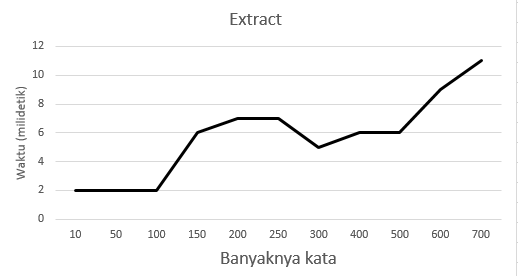
\includegraphics[scale=0.8]{Gambar/graf-extract}
	\caption{Grafik waktu yang dibutuhkan \textit{extract stego-object}} 
	\label{fig:graf-extract}
\end{figure}

Dapat dilihat pada Gambar \ref{fig:graf-extract} grafik perbandingan antara waktu yang dibutuhkan untuk \textit{extract}. Waktu yang dibutuhkan untuk melakukan ekstraksi memang berbanding lurus dengan banyak kata pada \textit{stego-object}, namun perbedaannya pun tidak terlalu jauh.

\begin{figure}[H]
	\centering
	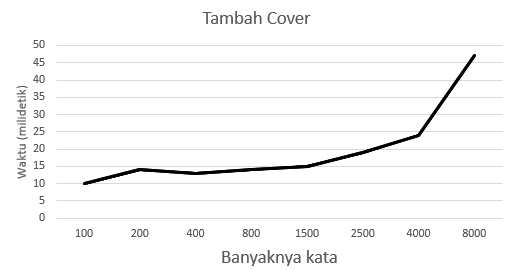
\includegraphics[scale=0.8]{Gambar/graf-tambah-cover}
	\caption{Grafik waktu yang dibutuhkan untuk menambahkan \textit{cover}} 
	\label{fig:graf-tambah-cover}
\end{figure}

Gambar \ref{fig:graf-tambah-cover} menunjukkan bahwa waktu yang dibutuhkan untuk menambahkan \textit{cover} tidaklah lama, karena perangkat hanya membuat \textit{file} baru dan menulis apa yang dimasukkan pengguna. Jika dilihat dari tiga grafik di atas, waktu yang paling lama adalah proses \textit{embed}, dikarenakan selain memenggal kata, proses \textit{embed} juga harus membaca \textit{file} kamus sinonim untuk memodifikasi \textit{stego-cover}.

\begin{figure}[H]
	\centering
	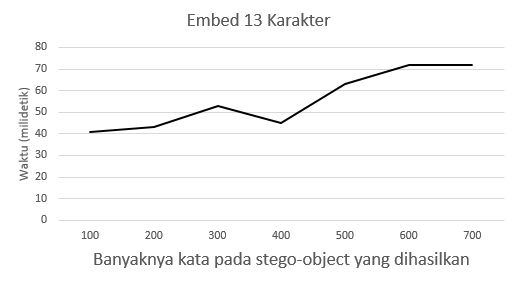
\includegraphics[scale=0.8]{Gambar/graf-embed-13-karakter}
	\caption{Grafik waktu yang dibutuhkan untuk \textit{embed} 13 karakter pesan rahasia} 
	\label{fig:graf-embed-13-karakter}
\end{figure}

\begin{figure}[H]
	\centering
	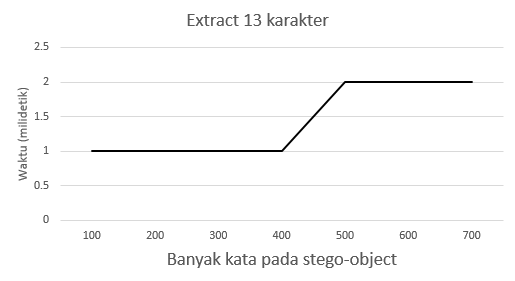
\includegraphics[scale=0.8]{Gambar/graf-extract-13-karakter}
	\caption{Grafik waktu yang dibutuhkan untuk \textit{extract} 13 karakter pesan rahasia} 
	\label{fig:graf-extract-13-karakter}
\end{figure}

Dapat dilihat pada Gambar \ref{fig:graf-embed-13-karakter} adalah grafik waktu yang dibutuhkan perangkat lunak untuk \textit{embed} pesan rahasia sepanjang 13 karakter ke dalam \textit{stego-cover} dengan panjang yang berbeda-beda. Pada Gambar \ref{fig:graf-extract-13-karakter} dapat dilihat grafik waktu yang dibutuhkan perangkat lunak untuk \textit{extract} pesan rahasia sepanjang 13 karakter dari \textit{stego-object} dengan panjang yang berbeda-beda pula.

Dari grafik dapat disimpulkan bahwa memang ada perbedaan waktu antara \textit{embed} ke dalam \textit{stego-cover} dengan panjang yang berbeda, walaupun panjang pesan rahasia sama. Seperti yang telah dijelaskan sebelumnya, proses \textit{embed} selalu membutuhkan waktu yang lebih lama dari proses \textit{extract}, hal ini juga dapat dilihat pada Gambar \ref{fig:graf-embed-13-karakter} dan \ref{fig:graf-extract-13-karakter}.

\begin{figure}[H]
	\centering
	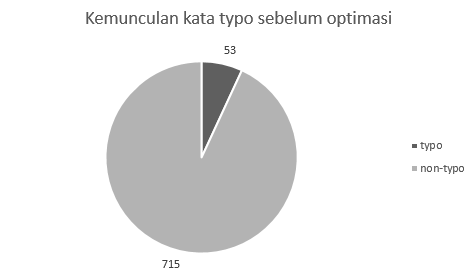
\includegraphics[scale=0.8]{Gambar/graf-typo-before}
	\caption{Grafik kemunculan kata \textit{typo} sebelum optimasi} 
	\label{fig:graf-typo-before}
\end{figure}

Pada Gambar \ref{fig:graf-typo-before} dapat dilihat bahwa kemunculan kata \textit{typo} pada \textit{stego-object} ada 53 kata dari total 771 kata. Pemakaian \textit{typo} sebagai sinonim tadinya digunakan baik untuk kata yang memiliki maupun tidak memiliki sinonim dengan nilai \textit{c}(\textit{w}) yang berebeda, dengan tujuan memperbanyak variasi kata untuk satu \textit{stego-object}. Namun karena dinilai akan menimbulkan kecurigaan, maka akan dilakukan optimasi terhadap kamus sinonim. Optimasi dilakukan atas dasar beberapa pertimbangan. \textit{Stego-cover} yang digunakan mengandung cukup banyak kata. Pemakaian kata dalam \textit{stego-cover} sudah cukup bervariasi. Maka dari itu diputuskan bahwa sinonim \textit{typo} hanya digunakan untuk kata yang benar-benar tidak memiliki sinonim dengan nilai \textit{c}(\textit{w}) yang berbeda dengan katanya. Grafik kemunculan kata \textit{typo} setelah optimasi dapat dilihat pada Gambar \ref{fig:graf-typo-after}.

\begin{figure}[H]
	\centering
	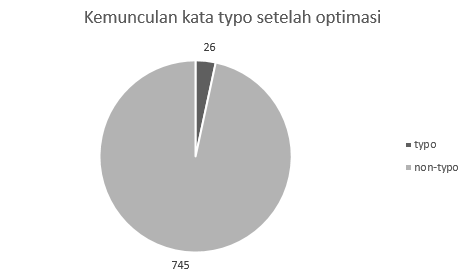
\includegraphics[scale=0.8]{Gambar/graf-typo-after}
	\caption{Grafik kemunculan kata \textit{typo} setelah optimasi} 
	\label{fig:graf-typo-after}
\end{figure}}{}
\ifdefstring{\vbabf}{1}{\chapter{Kesimpulan dan Saran}
\section{Kesimpulan}
Dari pembuatan perangkat lunak untuk menyembunyikan pesan rahasia dengan menggunakan steganografi berbasis suku kata bahasa Indonesia didapatkan kesimpulan sebagai berikut:
\begin{enumerate}
	\item Algoritma penyisipan dengan memanfaatkan \textit{c}(\textit{w}) dan kamus sinonim memungkinkan suatu \textit{stego-cover} dapat dipakai untuk segala pesan rahasia dengan syarat, kapasitas \textit{stego-cover} dapat menampung pesan rahasia.
	\item Implementasi dilakukan pada bahasa pemrograman Java. Dengan menggunakan bantuan \textit{File Reader}, perangkat lunak dapat mencari sinonim dari kata yang dibutuhkan.
	\item Performa yang dihasilkan perangkat lunak termasuk baik, karena pesan rahasia memang seharusnya tidak terlalu panjang.
	\item Fungsi pemenggalan kata pada perangkat lunak ini memang tidak sempurna, namun hal ini tidak dilihat sebagai kekurangan. Hal ini justru dapat mempersulit penyerang untuk mendapatkan pesan rahasia.
	\item Optimasi terhadap kamus sinonim dapat menurunkan frekuensi kemunculan kata \textit{typo} pada \textit{stego-object} secara signifikan. Hal ini dapat menurunkan tingkat kecurigaan pihak yang tidak bersangkutan saat membaca \textit{stego-object}.
	
\end{enumerate}

\section{Saran}
Saran yang dapat diberikan oleh penulis adalah:
\begin{enumerate}
	\item Memperbanyak karakter yang dapat disembunyikan oleh perangkat lunak.
	\item Mengurutkan penyimpanan kata pada kamus sinonim berdasarkan abjad, untuk mengoptimalkan waktu proses pencarian sinonim.
	\item Memperbaiki algoritma agar pola karakter spasi lebih sulit ditebak.
\end{enumerate}}{}
\ifdefstring{\vbabg}{1}{\include{Bab/bab7}}{}
\ifdefstring{\vbabh}{1}{\include{Bab/bab8}}{}
\ifdefstring{\vbabi}{1}{\include{Bab/bab9}}{}

\bibliographystyle{ieeetr}
\bibliography{pustaka}

\appendix
\apptoc

\tampillmp{\vlmp}
\ifdefstring{\vlmpa}{1}{\include{Lampiran/lampA}}{}
\ifdefstring{\vlmpb}{1}{\include{Lampiran/lampB}}{}
\ifdefstring{\vlmpc}{1}{\include{Lampiran/lampC}}{}
\ifdefstring{\vlmpd}{1}{\include{Lampiran/lampD}}{}
\ifdefstring{\vlmpe}{1}{\include{Lampiran/lampE}}{}
\ifdefstring{\vlmpf}{1}{\include{Lampiran/lampF}}{}
\ifdefstring{\vlmpg}{1}{\include{Lampiran/lampG}}{}
\ifdefstring{\vlmph}{1}{\include{Lampiran/lampH}}{}
\ifdefstring{\vlmpi}{1}{\include{Lampiran/lampI}}{}

\end{document}
